\documentclass[10pt, conference, compsocconf]{IEEEtran}

%\usepackage[numbers, sort, compress]{natbib}
\usepackage{graphicx}
\usepackage{amsmath}
\usepackage{amssymb}
\usepackage{color}
\usepackage{ifpdf}
%\usepackage{mdwlist}

%\usepackage{dcolumn}
\usepackage{float}
\usepackage[utf8]{inputenc}
\usepackage{multirow}
\usepackage{rotating}
\usepackage{subfigure}

\usepackage{moresize}
%\usepackage{setspace}

%\usepackage[numbers, sort, compress]{natbib}
%\usepackage{latex8}
%\usepackage{float}
%\usepackage{times}    
\usepackage{url}
\usepackage{booktabs}
\usepackage{listings}   
\usepackage{paralist}    
\usepackage{wrapfig}    
%\usepackage[footnotesize,it]{caption}
\usepackage{multirow}
\usepackage{ifpdf}
%\usepackage{srcltx}
%\usepackage{subfigure}
\usepackage{xspace}
\usepackage{keyval}  
\usepackage{color}

\definecolor{listinggray}{gray}{0.95}
\definecolor{darkgray}{gray}{0.7}
\definecolor{commentgreen}{rgb}{0, 0.4, 0}
\definecolor{darkblue}{rgb}{0, 0, 0.4}
\definecolor{middleblue}{rgb}{0, 0, 0.7}
\definecolor{darkred}{rgb}{0.4, 0, 0}
\definecolor{brown}{rgb}{0.5, 0.5, 0}
\definecolor{dkgreen}{rgb}{0,0.5,0}
\definecolor{orange}{rgb}{1,.5,0}
\definecolor{dandelion}{cmyk}{0,0.29,0.84,0}

\usepackage[normalem]{ulem}
\makeatletter
\def\cyanuwave{\bgroup \markoverwith{\lower3.5\p@\hbox{\sixly \textcolor{cyan}{\char58}}}\ULon}
\def\reduwave{\bgroup \markoverwith{\lower3.5\p@\hbox{\sixly \textcolor{red}{\char58}}}\ULon}
\def\blueuwave{\bgroup \markoverwith{\lower3.5\p@\hbox{\sixly \textcolor{blue}{\char58}}}\ULon}
\font\sixly=lasy6 % does not re-load if already loaded, so no memory problem.
\makeatother


%\usepackage{xcolor}
\newif\ifdraft
\drafttrue
\ifdraft
 \newcommand{\N}[1]{\textbf{NOTE: #1}\xspace}
 \newcommand{\jhanote}[1]{ {\textcolor{red} { ***SJ: #1 }}}
 \newcommand{\katznote}[1]{ {\textcolor{blue} { ***DSK: #1 }}}
 \newcommand{\mtnote}[1]{ {\textcolor{orange} { ***MT: #1 }}}
 \newcommand{\jonnote}[1]{ {\textcolor{dkgreen} { ***JW: #1 }}}
  \newcommand{\aanote}[1]{ {\textcolor{dkgreen} { ***AA: #1 }}}
 \newcommand{\note}[1]{ {\textcolor{brown} { *** #1 }}}
\else
 \newcommand{\N}[1]{}
 \newcommand{\jhanote}[1]{}
 \newcommand{\katznote}[1]{}
 \newcommand{\mtnote}[1]{}
 \newcommand{\jonnote}[1]{}
 \newcommand{\note}[1]{}
\fi

\newif\ifdraft
%\drafttrue
\ifdraft
\newcommand{\terminology}[1]{ {\textcolor{red} {(Terminology used: \textbf{#1}) }}}
\newcommand{\owave}[1]{ {\cyanuwave{#1}}}
\newcommand{\jwave}[1]{ {\reduwave{#1}}}
\newcommand{\alwave}[1]{ {\blueuwave{#1}}}
\newcommand{\alnote}[1]{ {\textcolor{blue} { ***andreL: #1 }}}
\newcommand{\amnote}[1]{ {\textcolor{blue} { ***andreM: #1 }}}
\newcommand{\smnote}[1]{ {\textcolor{brown} { ***sharath: #1 }}}
\newcommand{\pmnote}[1]{ {\textcolor{brown} { ***Pradeep: #1 }}}
\newcommand{\msnote}[1]{ {\textcolor{cyan} { ***mark: #1 }}}
\newcommand{\mrnote}[1]{ {\textcolor{purple} { ***melissa: #1 }}}
%\newcommand{\mtnote}[1]{ {\textcolor{orange} { ***matteo: #1 }}}
\else
\newcommand{\onote}[1]{}
\newcommand{\terminology}[1]{}
\newcommand{\owave}[1]{#1}
\newcommand{\jwave}[1]{#1}
\newcommand{\alnote}[1]{}
\newcommand{\amnote}[1]{}
\newcommand{\athotanote}[1]{}
\newcommand{\smnote}[1]{}
\newcommand{\pmnote}[1]{}
\newcommand{\msnote}[1]{}
\newcommand{\mrnote}[1]{}
\newcommand{\aznote}[1]{}
%\newcommand{\mtnote}[1]{}
\fi

\newcommand{\cloud}{cloud\xspace}
\newcommand{\clouds}{clouds\xspace}
\newcommand{\pilot}{Pilot\xspace}
\newcommand{\pilots}{Pilots\xspace}
\newcommand{\pilotjob}{Pilot-Job\xspace}
\newcommand{\pilotjobs}{Pilot-Jobs\xspace}
\newcommand{\pilotcompute}{Pilot-Compute\xspace}
\newcommand{\pilotcomputedescription}{Pilot-Compute Description\xspace}
\newcommand{\pilotdescription}{Pilot-Description\xspace}
\newcommand{\pilotcomputes}{Pilot-Computes\xspace}
\newcommand{\pilotdata}{Pilot-Data\xspace}
\newcommand{\pilotdatadescription}{Pilot-Data Description\xspace}
\newcommand{\pilotdataservice}{Pilot-Data Service\xspace}
\newcommand{\pilotcomputeservice}{Pilot-Compute Service\xspace}
\newcommand{\computedataservice}{Compute-Data Service\xspace}
\newcommand{\computeunitdescription}{Compute-Unit Description\xspace}
\newcommand{\dataunitdescription}{Data-Unit Description\xspace}
\newcommand{\pilotmapreduce}{PilotMapReduce\xspace}
\newcommand{\mrmg}{MR-Manager\xspace}
\newcommand{\pstar}{P*\xspace}
\newcommand{\pd}{PD\xspace}
\newcommand{\pc}{PC\xspace}
\newcommand{\pcs}{PCs\xspace}
\newcommand{\pj}{PJ\xspace}
\newcommand{\pjs}{PJs\xspace}
\newcommand{\pds}{Pilot Data Service\xspace}
\newcommand{\computeunit}{Compute-Unit\xspace}
\newcommand{\computeunits}{Compute-Units\xspace}
\newcommand{\dataunit}{Data-Unit\xspace}
\newcommand{\dataunits}{Data-Units\xspace}
\newcommand{\du}{DU\xspace}
\newcommand{\dus}{DUs\xspace}
\newcommand{\dud}{DUD\xspace}
\newcommand{\cu}{CU\xspace}
\newcommand{\cus}{CUs\xspace}
\newcommand{\cud}{CUD\xspace}
\newcommand{\su}{SU\xspace}
\newcommand{\sus}{SUs\xspace}
\newcommand{\schedulableunit}{Schedulable Unit\xspace}
\newcommand{\schedulableunits}{Schedulable Units\xspace}
\newcommand{\cc}{c\&c\xspace}
\newcommand{\CC}{C\&C\xspace}
\newcommand{\up}{\vspace*{-1em}}
\newcommand{\upp}{\vspace*{-0.5em}}
\newcommand{\numrep}{8 }
\newcommand{\samplenum}{4 }
\newcommand{\tmax}{$T_{max}$ }
\newcommand{\tc}{$T_{C}$ }
\newcommand{\tcnsp}{$T_{C}$}
\newcommand{\bj}{BigJob\xspace}
\newcommand{\irods}{iRODS\xspace}

\newcommand{\I}[1]{\textit{#1}\xspace}
\newcommand{\B}[1]{\textbf{#1}\xspace}
\newcommand{\T}[1]{\texttt{#1}\xspace}
\newcommand{\C}[1]{\textsc{#1}\xspace}

\newcommand{\mr}[1]{\multirow{2}{*}{#1}}%
\newcommand{\mc}[2]{\multicolumn{#1}{l}{#2}}

\lstdefinestyle{myListing}{
  frame=single,   
  backgroundcolor=\color{listinggray},  
  %float=t,
  language=C,       
  basicstyle=\ttfamily \footnotesize,
  breakautoindent=true,
  breaklines=true
  tabsize=2,
  captionpos=b,  
  aboveskip=0em,
  belowskip=-2em,
  %numbers=left, 
  %numberstyle=\tiny
}      

\lstdefinestyle{myPythonListing}{
  frame=single,   
  backgroundcolor=\color{listinggray},  
  %float=t,
  language=Python,       
  basicstyle=\ttfamily \scriptsize,
  breakautoindent=true,
  breaklines=true
  tabsize=2,
  captionpos=b,  
  %numbers=left, 
  %numberstyle=\tiny
}



%  \setlength{\parskip}{0.05ex} % 1ex plus 0.5ex minus 0.2ex}
%  \setlength{\parsep}{0pt}
%  %\setlength{\headsep}{0pt}
%  \setlength{\topskip}{0pt}
%  \setlength{\topmargin}{0pt}
%  %\setlength{\topsep}{0pt}
%  \setlength{\partopsep}{0pt}

% This is now the recommended way for checking for PDFLaTeX:


\ifpdf
\DeclareGraphicsExtensions{.pdf, .jpg, .tif}
\else
\DeclareGraphicsExtensions{.ps,  .eps, .jpg}
\fi

\tolerance=1000
\hyphenpenalty=10


\usepackage{listings}
\usepackage{comment}

% Some very useful LaTeX packages include:
% (uncomment the ones you want to load)

% *** MISC UTILITY PACKAGES ***
%
%\usepackage{ifpdf}
% Heiko Oberdiek's ifpdf.sty is very useful if you need conditional
% compilation based on whether the output is pdf or dvi.
% usage:
% \ifpdf
%   % pdf code
% \else
%   % dvi code
% \fi
% The latest version of ifpdf.sty can be obtained from:
% http://www.ctan.org/tex-archive/macros/latex/contrib/oberdiek/
% Also, note that IEEEtran.cls V1.7 and later provides a builtin
% \ifCLASSINFOpdf conditional that works the same way.
% When switching from latex to pdflatex and vice-versa, the compiler may
% have to be run twice to clear warning/error messages.

% *** CITATION PACKAGES ***
%
%\usepackage{cite}
% cite.sty was written by Donald Arseneau
% V1.6 and later of IEEEtran pre-defines the format of the cite.sty package
% \cite{} output to follow that of IEEE. Loading the cite package will
% result in citation numbers being automatically sorted and properly
% "compressed/ranged". e.g., [1], [9], [2], [7], [5], [6] without using
% cite.sty will become [1], [2], [5]--[7], [9] using cite.sty. cite.sty's
% \cite will automatically add leading space, if needed. Use cite.sty's
% noadjust option (cite.sty V3.8 and later) if you want to turn this off.
% cite.sty is already installed on most LaTeX systems. Be sure and use
% version 4.0 (2003-05-27) and later if using hyperref.sty. cite.sty does
% not currently provide for hyperlinked citations.
% The latest version can be obtained at:
% http://www.ctan.org/tex-archive/macros/latex/contrib/cite/
% The documentation is contained in the cite.sty file itself.

% *** GRAPHICS RELATED PACKAGES ***
%
\ifCLASSINFOpdf
  % \usepackage[pdftex]{graphicx}
  % declare the path(s) where your graphic files are
  % \graphicspath{{../pdf/}{../jpeg/}}
  % and their extensions so you won't have to specify these with
  % every instance of \includegraphics
  % \DeclareGraphicsExtensions{.pdf,.jpeg,.png}
\else
  % or other class option (dvipsone, dvipdf, if not using dvips). graphicx
  % will default to the driver specified in the system graphics.cfg if no
  % driver is specified.
  % \usepackage[dvips]{graphicx}
  % declare the path(s) where your graphic files are
  % \graphicspath{{../eps/}}
  % and their extensions so you won't have to specify these with
  % every instance of \includegraphics
  % \DeclareGraphicsExtensions{.eps}
\fi
% graphicx was written by David Carlisle and Sebastian Rahtz. It is
% required if you want graphics, photos, etc. graphicx.sty is already
% installed on most LaTeX systems. The latest version and documentation can
% be obtained at:
% http://www.ctan.org/tex-archive/macros/latex/required/graphics/
% Another good source of documentation is "Using Imported Graphics in
% LaTeX2e" by Keith Reckdahl which can be found as epslatex.ps or
% epslatex.pdf at: http://www.ctan.org/tex-archive/info/
%
% latex, and pdflatex in dvi mode, support graphics in encapsulated
% postscript (.eps) format. pdflatex in pdf mode supports graphics
% in .pdf, .jpeg, .png and .mps (metapost) formats. Users should ensure
% that all non-photo figures use a vector format (.eps, .pdf, .mps) and
% not a bitmapped formats (.jpeg, .png). IEEE frowns on bitmapped formats
% which can result in "jaggedy"/blurry rendering of lines and letters as
% well as large increases in file sizes.
%
% You can find documentation about the pdfTeX application at:
% http://www.tug.org/applications/pdftex

% *** MATH PACKAGES ***
%
%\usepackage[cmex10]{amsmath}
% A popular package from the American Mathematical Society that provides
% many useful and powerful commands for dealing with mathematics. If using
% it, be sure to load this package with the cmex10 option to ensure that
% only type 1 fonts will utilized at all point sizes. Without this option,
% it is possible that some math symbols, particularly those within
% footnotes, will be rendered in bitmap form which will result in a
% document that can not be IEEE Xplore compliant!
%
% Also, note that the amsmath package sets \interdisplaylinepenalty to 10000
% thus preventing page breaks from occurring within multiline equations. Use:
%\interdisplaylinepenalty=2500
% after loading amsmath to restore such page breaks as IEEEtran.cls normally
% does. amsmath.sty is already installed on most LaTeX systems. The latest
% version and documentation can be obtained at:
% http://www.ctan.org/tex-archive/macros/latex/required/amslatex/math/

% *** SPECIALIZED LIST PACKAGES ***
%
%\usepackage{algorithmic}
% algorithmic.sty was written by Peter Williams and Rogerio Brito.
% This package provides an algorithmic environment fo describing algorithms.
% You can use the algorithmic environment in-text or within a figure
% environment to provide for a floating algorithm. Do NOT use the algorithm
% floating environment provided by algorithm.sty (by the same authors) or
% algorithm2e.sty (by Christophe Fiorio) as IEEE does not use dedicated
% algorithm float types and packages that provide these will not provide
% correct IEEE style captions. The latest version and documentation of
% algorithmic.sty can be obtained at:
% http://www.ctan.org/tex-archive/macros/latex/contrib/algorithms/
% There is also a support site at:
% http://algorithms.berlios.de/index.html
% Also of interest may be the (relatively newer and more customizable)
% algorithmicx.sty package by Szasz Janos:
% http://www.ctan.org/tex-archive/macros/latex/contrib/algorithmicx/

% *** ALIGNMENT PACKAGES ***
%
%\usepackage{array}
% Frank Mittelbach's and David Carlisle's array.sty patches and improves
% the standard LaTeX2e array and tabular environments to provide better
% appearance and additional user controls. As the default LaTeX2e table
% generation code is lacking to the point of almost being broken with
% respect to the quality of the end results, all users are strongly
% advised to use an enhanced (at the very least that provided by array.sty)
% set of table tools. array.sty is already installed on most systems. The
% latest version and documentation can be obtained at:
% http://www.ctan.org/tex-archive/macros/latex/required/tools/

%\usepackage{mdwmath}
%\usepackage{mdwtab}
% Also highly recommended is Mark Wooding's extremely powerful MDW tools,
% especially mdwmath.sty and mdwtab.sty which are used to format equations
% and tables, respectively. The MDWtools set is already installed on most
% LaTeX systems. The lastest version and documentation is available at:
% http://www.ctan.org/tex-archive/macros/latex/contrib/mdwtools/

% IEEEtran contains the IEEEeqnarray family of commands that can be used to
% generate multiline equations as well as matrices, tables, etc., of high
% quality.

%\usepackage{eqparbox}
% Also of notable interest is Scott Pakin's eqparbox package for creating
% (automatically sized) equal width boxes - aka "natural width parboxes".
% Available at:
% http://www.ctan.org/tex-archive/macros/latex/contrib/eqparbox/

% *** SUBFIGURE PACKAGES ***
%\usepackage[tight,footnotesize]{subfigure}
% subfigure.sty was written by Steven Douglas Cochran. This package makes it
% easy to put subfigures in your figures. e.g., "Figure 1a and 1b". For IEEE
% work, it is a good idea to load it with the tight package option to reduce
% the amount of white space around the subfigures. subfigure.sty is already
% installed on most LaTeX systems. The latest version and documentation can
% be obtained at:
% http://www.ctan.org/tex-archive/obsolete/macros/latex/contrib/subfigure/
% subfigure.sty has been superceeded by subfig.sty.

%\usepackage[caption=false]{caption}
%\usepackage[font=footnotesize]{subfig}
% subfig.sty, also written by Steven Douglas Cochran, is the modern
% replacement for subfigure.sty. However, subfig.sty requires and
% automatically loads Axel Sommerfeldt's caption.sty which will override
% IEEEtran.cls handling of captions and this will result in nonIEEE style
% figure/table captions. To prevent this problem, be sure and preload
% caption.sty with its "caption=false" package option. This is will preserve
% IEEEtran.cls handing of captions. Version 1.3 (2005/06/28) and later
% (recommended due to many improvements over 1.2) of subfig.sty supports
% the caption=false option directly:
%\usepackage[caption=false,font=footnotesize]{subfig}
%
% The latest version and documentation can be obtained at:
% http://www.ctan.org/tex-archive/macros/latex/contrib/subfig/
% The latest version and documentation of caption.sty can be obtained at:
% http://www.ctan.org/tex-archive/macros/latex/contrib/caption/

% *** FLOAT PACKAGES ***
%
%\usepackage{fixltx2e}
% fixltx2e, the successor to the earlier fix2col.sty, was written by
% Frank Mittelbach and David Carlisle. This package corrects a few problems
% in the LaTeX2e kernel, the most notable of which is that in current
% LaTeX2e releases, the ordering of single and double column floats is not
% guaranteed to be preserved. Thus, an unpatched LaTeX2e can allow a
% single column figure to be placed prior to an earlier double column
% figure. The latest version and documentation can be found at:
% http://www.ctan.org/tex-archive/macros/latex/base/

%\usepackage{stfloats}
% stfloats.sty was written by Sigitas Tolusis. This package gives LaTeX2e
% the ability to do double column floats at the bottom of the page as well
% as the top. (e.g., "\begin{figure*}[!b]" is not normally possible in
% LaTeX2e). It also provides a command:
%\fnbelowfloat
% to enable the placement of footnotes below bottom floats (the standard
% LaTeX2e kernel puts them above bottom floats). This is an invasive package
% which rewrites many portions of the LaTeX2e float routines. It may not work
% with other packages that modify the LaTeX2e float routines. The latest
% version and documentation can be obtained at:
% http://www.ctan.org/tex-archive/macros/latex/contrib/sttools/
% Documentation is contained in the stfloats.sty comments as well as in the
% presfull.pdf file. Do not use the stfloats baselinefloat ability as IEEE
% does not allow \baselineskip to stretch. Authors submitting work to the
% IEEE should note that IEEE rarely uses double column equations and
% that authors should try to avoid such use. Do not be tempted to use the
% cuted.sty or midfloat.sty packages (also by Sigitas Tolusis) as IEEE does
% not format its papers in such ways.

% *** PDF, URL AND HYPERLINK PACKAGES ***
%
%\usepackage{url}
% url.sty was written by Donald Arseneau. It provides better support for
% handling and breaking URLs. url.sty is already installed on most LaTeX
% systems. The latest version can be obtained at:
% http://www.ctan.org/tex-archive/macros/latex/contrib/misc/
% Read the url.sty source comments for usage information. Basically,
% \url{my_url_here}.

% *** Do not adjust lengths that control margins, column widths, etc. ***
% *** Do not use packages that alter fonts (such as pslatex).         ***
% There should be no need to do such things with IEEEtran.cls V1.6 and later.
% (Unless specifically asked to do so by the journal or conference you plan
% to submit to, of course. )

% correct bad hyphenation here
\hyphenation{op-tical net-works semi-conduc-tor}

% -----------------------------------------------------------------------------
% BEGIN DOCUMENT
% -----------------------------------------------------------------------------
\begin{document}

\title{Everything you wanted to know about PanDA but were truly truly afraid to
ask}


% author names and affiliations
% use a multiple column layout for up to two different
% affiliations
\author{\IEEEauthorblockN{Authors Name/s per 1st Affiliation (Author)}
\IEEEauthorblockA{line 1 (of Affiliation): dept.\ name of organization\\
line 2: name of organization, acronyms acceptable\\
line 3: City, Country\\
line 4: Email: name@xyz.com}
\and
\IEEEauthorblockN{Authors Name/s per 2nd Affiliation (Author)}
\IEEEauthorblockA{line 1 (of Affiliation): dept.\ name of organization\\
line 2: name of organization, acronyms acceptable\\
line 3: City, Country\\
line 4: Email: name@xyz.com}
}

% conference papers do not typically use \thanks and this command
% is locked out in conference mode. If really needed, such as for
% the acknowledgment of grants, issue a \IEEEoverridecommandlockouts
% after \documentclass

% for over three affiliations, or if they all won't fit within the width
% of the page, use this alternative format:
%
%\author{\IEEEauthorblockN{Michael Shell\IEEEauthorrefmark{1},
%Homer Simpson\IEEEauthorrefmark{2},
%James Kirk\IEEEauthorrefmark{3},
%Montgomery Scott\IEEEauthorrefmark{3} and
%Eldon Tyrell\IEEEauthorrefmark{4}}
%\IEEEauthorblockA{\IEEEauthorrefmark{1}School of Electrical and Computer Engineering\\
%Georgia Institute of Technology,
%Atlanta, Georgia 30332--0250\\ Email: see http://www.michaelshell.org/contact.html}
%\IEEEauthorblockA{\IEEEauthorrefmark{2}Twentieth Century Fox, Springfield, USA\\
%Email: homer@thesimpsons.com}
%\IEEEauthorblockA{\IEEEauthorrefmark{3}Starfleet Academy, San Francisco, California 96678-2391\\
%Telephone: (800) 555--1212, Fax: (888) 555--1212}
%\IEEEauthorblockA{\IEEEauthorrefmark{4}Tyrell Inc., 123 Replicant Street, Los Angeles, California 90210--4321}}

% use for special paper notices
%\IEEEspecialpapernotice{(Invited Paper)}

% make the title area
\maketitle

% ----------------------------------------------------------------------------
% ABSTRACT
% ----------------------------------------------------------------------------
\begin{abstract}
Experiments at the Large Hadron Collider (LHC) face unprecedented computing
challenges. Heterogeneous resources are distributed worldwide, thousands of
physicists analyzing the data need remote access to hundreds of computing
sites, the volume of processed data is beyond the exabyte scale, and data
processing requires more than billions of hours of computing usage per year. The
PanDA (Production and Distributed Analysis) system was developed to meet the
scale and complexity of LHC distributed computing for the ATLAS experiment. In
the process, the old batch job paradigm of computing in HEP was discarded in
favor of a far more flexible and scalable model. The success of PanDA at the LHC
is leading to widespread adoption and testing by other experiments. PanDA is
the first exascale workload management system in HEP, already operating at
a million computing jobs per day, and processing over an exabyte of data in
2013. We will describe the design and implementation of PanDA, present data on
the performance of PanDA at the LHC, and discuss plans for future evolution
of the system to meet new challenges of scale, heterogeneity and increasing
user base.
\end{abstract}

\begin{IEEEkeywords}
TBD\@.
\end{IEEEkeywords}


% For peer review papers, you can put extra information on the cover
% page as needed:
% \ifCLASSOPTIONpeerreview
% \begin{center} \bfseries EDICS Category: 3-BBND \end{center}
% \fi
%
% For peerreview papers, this IEEEtran command inserts a page break and
% creates the second title. It will be ignored for other modes.
\IEEEpeerreviewmaketitle


% ----------------------------------------------------------------------------
% I - INTRODUCTION
% ----------------------------------------------------------------------------
\section{Introduction}\label{sec:intro}

The Large Hadron Collider (LHC) is created to explore the fundamental properties
of matter for the next decades. Since LHC start-up in 2009, the experiments
collected and distributed hundreds of petabytes of data worldwide to hundreds of
computer centers. Thousands of physicists analyze petascale data volumes daily.
One of the LHC experiments, the ATLAS~\cite{Aad:2008}, utilizes the Production
and Distributed Analysis (PanDA) workload management system~\cite{Maeno2011}
(WMS) for distributed data processing and analysis. The ATLAS Computing
model~\cite{Atlas2005} is based on a Grid paradigm~\cite{Foster:1998}, with
multilevel, hierarchically distributed computing and storage resources. PanDA
has been developed to meet growing ATLAS production and analysis requirements
for a data-driven workload management system capable of operating at LHC data
processing scale.

PanDA has a highly scalable architecture. Scalability has been demonstrated in
ATLAS through the rapid increase in usage over the past several years of
operations, and PanDA is expected to meet the continuously growing computing
requirements of ATLAS over the next decade. PanDA was designed to have the
flexibility to adapt to emerging computing technologies in processing, storage,
networking as well as the underlying software stack. This flexibility has also
been successfully demonstrated through the past six years: computing centers in
ATLAS, spanning many continents, were seamlessly integrated into PanDA\@.

PanDA manages a wide spectrum of workloads, ranging from raw data processing to
Monte Carlo simulation and user analysis, while constantly evolving to meet
rapidly changing science needs. Today, PanDA serves several thousand users,
managing job distribution to hundreds of ATLAS sites with more than 100,000 CPU
cores which process more than a million jobs per day (Figure~\ref{fig:daily}).

\begin{figure}
    \begin{center}
        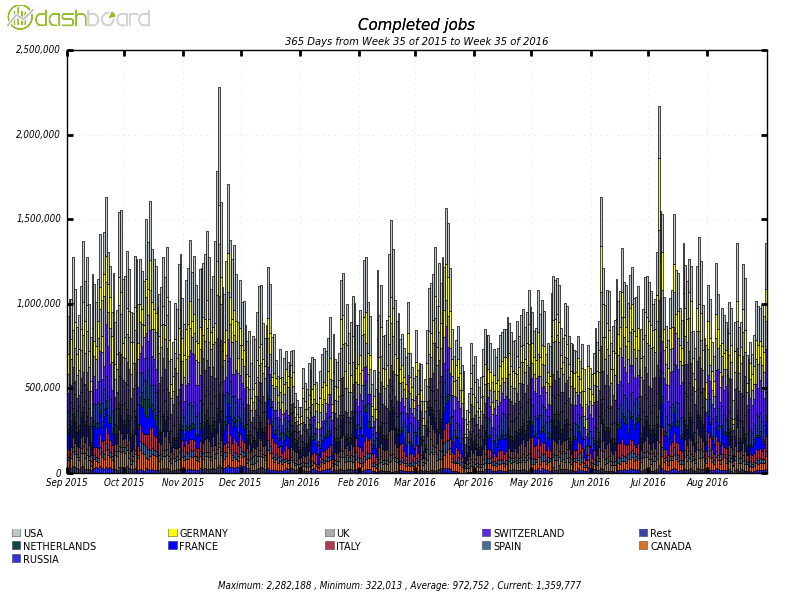
\includegraphics[width=\columnwidth]{figures/DailyJobs.png}
        \caption{Daily completed jobs on ATLAS Grid for the past 12 month}
    \end{center}
\label{fig:daily}
\end{figure}

In this paper, we describe how PanDA has been engineered to execute a specific
stage of the ATLAS Monte Carlo workflow on Titan, the larger high-performance
computing HPC system currently available in the USA\@.\mtnote{Explain the
benefits offered by Titan in terms of multithreading per node and possibly large
amount of concurrent nodes. Introduce also the notion of backfill.} This extends
the scope of PanDA's compute model, integrating both high-throughput and
high-performance computing resources and enabling the concurrent execution of
both  single and multi-core jobs. The integration of PanDA and Titan went
through three main engineering phases: (i) feasibility study and rapid
prototyping of an initial solution; (ii) progressing scaling of the  prototype
to saturate the available resources; (iii) study of a product-grade architecture
for generic HPC resources. Both phase i and ii have been completed enabling the
execution of up to eight million jobs a week on Titan. A prototype has been
engineered to support phase iii and experimental data are being collected.

In the next section we introduce \ldots.


\begin{enumerate}
  \item Problem that has been solved: executing many applications on
  heterogeneous distributed resources.
  \item Why are WMS needed?
  \item Increasing importance of WMS w.r.t complex and scalable applications on
  heterogeneous distributed resources.
  \item \ldots
  \item Overview/Summary of paper.
\end{enumerate}


% ----------------------------------------------------------------------------
% II - BACKGROUND AND RELATED WORK
% ----------------------------------------------------------------------------
\section{Background and Related Work}
\label{sec:bkgrd}

\begin{enumerate}
  \item Brief overview of distributed CI\@.
  \item Workload vs Workflow. (DONE)
  \item Distinguish between WFMS and WLMS\@.
  \begin{enumerate}
    \item Role of Workload MS\@: help ``hide'' and federate heterogeneous resources.
  \end{enumerate}
\end{enumerate}

% Please do not correct bckground to background.
% \jhanote{In this section we should talk less about PanDA and more about other
% WMS -- highlighting the fact that (i) there isn't a comprehensive systems
% (design, architecture and execution properties) discussion of other WMS so
% difficult to compare}\mtnote{Better?}


% \jhanote{(ii) real comparison should be to the Gliden-in WMS ecosystem and use
% this as opportunity to narrate the reasons for the divergence.}\mtnote{From our
% meetings with Sergey: Before Run 1, ATLAS management become uncomfortable with
% the pace at which other WMS were being developed, loosing trust in their ability
% to deliver production-grade capabilities. ATLAS USA decided to go solo and
% developed their own solution. PanDA proven to be able to deliver the
% usual pilot-based WMS capabilities at the right scale. For that, it was chosen
% over other solutions.}

% \jhanote{Also might this section be moved towards the rear, as this is  a
% practice paper and not a traditional research paper?}\mtnote{Done.}


Several pilot-enabled WMS were developed for the LHC experiments:
AliEn~\cite{Bagnasco2010} for ALICE; DIRAC~\cite{Paterson2010} for LHCb;
GlideinWMS~\cite{sfiligoi2008glideinwms} for CMS; and
PanDA~\cite{maeno2014evolution} for ATLAS. These systems implement similar
design and architectural principles: centralization of task and resource
management, and of monitoring and accounting; distribution of task execution
across multiple sites; unification of the application interface; hiding of
resource heterogeneity; and collection of static and sometimes dynamic
information about resources.

AliEn, DIRAC, GlideinWMS and PanDA all share a similar design with two types of
components: the management ones facing the application layer and centralizing
the capabilities required to acquire tasks' descriptions and matching them to
resource capabilities; and resource components used to acquire compute and data
resources and information about their capabilities. Architecturally, the
management components include one or more queue and a scheduler that coordinates
with the resource modules via push/pull protocols. All resource components
include middleware-specific APIs to request for resources, and a pilot capable
of pulling tasks from the management modules and executing them on its
resources.

AliEn, DIRAC, GlideinWMS and PanDA also have similar implementations. These WMS
were initially implemented to use Grid resources, using one or more components
to the Condor software ecosystem~\cite{thain2005distributed} and, as with
GlideinWMS, contributing to its development. Accordingly, all LHC WMS
implemented Grid-like authentication and authorization systems and adopted a
computational model based on distributing a large amount of single/few-cores
tasks across hundreds of sites\mtnote{Is this true?}.

All the experiments at LHC produces and process large amount of data both from
actual collisions in the accelerator and from their simulations. Dedicated,
multi-tiered data systems have been built to store, replicate, and distributed
these data. All LHC WMS interface with these systems to move data to the sites
where related compute tasks are executed or to schedule compute tasks where
(large amount of) data are already stored.

% -----------------------------------------------------------------------------
% NOTES ON TASK, JOBS, AND WORKFLOW TERMINOLOGY
% -----------------------------------------------------------------------------
% Currently, the implementation of PanDA WMS has at least two distinguishing
% features: the scale at which it operates distributed computing, and
% network-aware scheduling of tasks to sites\mtnote{PanDA team: please let me
% know whether more unique (i.e., not present in other LHC WMS) features of
% PanDA implementation should be indicated}. PanDA concurrently supports
% distributed computations on up to 240,000 cores, submitting more than 365
% million jobs a year across 100 sites, and processing up to XXXXPB of data
% distributed worldwide on XX Tier 1-3 facilities. As for 2017, PanDA serves
% several thousand users, including XX production groups. The scale of this
% operation is unprecedented, making PanDA the WMS that manages the largest
% computational campaign in the world.

% PanDA was initially implemented to support computations across an unreliable
% and relatively expensive networking infrastructure. Accordingly, PanDA
% assumed a rigid model of data placement based on replication and long-term
% storage of data on the Grid sites. This model proven too wasteful, requiring
% storage space for unused and obsolete data. PanDA implementation was evolved
% to benefit from the development of the internet and of the networking
% infrastructure for scientific research. Today, PanDA constantly monitors
% network throughput and latency among its management components, Grid sites and
% data facilities. PanDA uses this information to schedule tasks on sites,
% depending on the estimated time required to download and/or replicate input
% data and to stage out output data.

% The dynamic management of data replication and download is an example of a
% generalized paradigm shift that distinguishes the implementation of PanDA from
% other WMS. New components are being implemented to support: (i) dynamic sizing
% of input dataset based on resource capabilities; (ii) dynamic sizing of the
% resources held by pilots both in terms of number of cores and duration of the
% pilot; and (iii) further abstraction of different types of resources to
% reconcile high-throughput and high-performance computing paradigms.
% -----------------------------------------------------------------------------

% -----------------------------------------------------------------------------
% NOTES ON TASK, JOBS, AND WORKFLOW TERMINOLOGY
% -----------------------------------------------------------------------------
% Each task may have an arbitrary number of properties like number of cores,
% executables, or input/output files. Tasks may have precedence interrelations,
% depending on their data dependences or any other type of dependency mandated
% by the application algorithms. Tasks with precedence relations have to be
% executed serially; otherwise, tasks can be executed concurrently. A workload
% is defined as a set of tasks that can be executed concurrently. As such, a
% workflow can be composed of a set of workloads.

% The terms ``task'' and ``job'' are also used inconsistently across communities
% that perform scientific computing. In this paper, ``job'' refers to the unit
% of work that is submitted to a local resource management system (LRMS), like
% the Slurm or PBS batch system of a cluster. As such, a task can become a job
% when is scheduled on a resource that exposes a LRMS but can also become a
% virtual machine or a container when bootstrapped on an infrastructure
% supporting virtualization. Tasks can be statically or dynamically grouped
% into jobs, depending on the resource capabilities and the task requirements.

% Usually, workflows are represented as graphs in which tasks are vertices and
% relations are edges~\cite{}. Often, graphs are supposed to be acyclic but
% graphs with cycles have been used to represent workflows of
% workflows~\cite{}. In this paper, a workflow template is a type of graph
% while a workflow instance is a workflow template with specific vertices and
% edges. Further, a workflow instance is ``abstract'' when no resource
% properties are available for all vertices, ``concrete'' otherwise~\cite{}.
% When not qualified, the term ``workflow'' indicates a abstract workflow
% instance.

% Notes for refactoring:
% \begin{itemize}
%     \item Naming and nomenclature is a contribution
%     \item 1, 1.5 pages.
% \end{itemize}
% -----------------------------------------------------------------------------


\begin{enumerate}
  \item Other workload management systems (WMS) (not exclusive)
  \begin{enumerate}
    \item glidein-WMS
    \item Dirac
    \item ALICE-AlieN
  \end{enumerate}
  \begin{enumerate}
    \item Comparison and contrast
    \item Core features of a general WMS, i.e., minimal complete model of a WMS\@.
  \end{enumerate}
\end{enumerate}

\subsection{Alien}
Alien is a Workload and Data Management system composed of a 	set of middleware tools and services entirely based on web-services and standard protocols. Alien was originally developed for the ALICE experiment \cite{} but subsequently used by several virtual organizations \cite{}. 
%The system has been deployed in 2001 for distributed producti	on of Monte Carlo data, detector simulation and reconstruction.
Alien is composed of two type of services:
\begin{itemize}
\item
\emph{Central services}, these services are unique for each virtual organisation, therefore there is only one  configuration point for the management;
\item \emph{Site services}, they provide the interfacing to local resources and Grid services running on a VO-box;
\end{itemize}

The most important central services are:
\begin{itemize}
\item \emph{Job Manager}, a database that keeps track of all the jobs submitted to the system and their current execution status;
\item \emph{Brokers}, they are the core of task executions and data transfers; they receive tasks in form of JDL,  keep them ordered by priority and send them to the CE for execution;
\item \emph{Optimizers}, they are used to minimize the work of the Broker by scanning periodially the task queue and re-arranging the tasks in such a way that fairness and priority policies are guaranted;
\item \emph{Data Catalogue}, it keeps track of the scripts and files uploaded on Storage Elements.
\end{itemize}

%The Computing Agents are instead site services that monitor the local Computing Element, advertise site's capabilities and are responsible for submitting the JobAgents.

%Information about the status of the sites and central services, full job statistics and monitoring information are kept in a MonALISA repository.
%% CLUSTER MONITOR SHOULD BE EQUAL TO COMPUTING AGENT
%% Job Manager should be equal to TaskQueue
%% Process Monitor == PIlot????

The job execution in Alien is usually distributed over several sites. Each of these sites has at least one service called ClusterMonitor. On one side the Cluster Monitor is used to communicate with Central services (Job Manager and Broker), on the other side it can manage Computing Elements (CE) by starting and stopping them whenever it receives the signal.
The CE is the resource in charge of the execution of the jobs. A CE usually is associated with a batch queue and can send the jobs to the worker nodes controlled by the queue.

The CE asks the Broker for jobs to execute by sending its JDL. Once received the JDL, the Broker will try to match it with the JDL of the jobs in queue. If a match exists then the Broker sends the jobs JDL to the CE.
Immediately after receving a job JDL, the CE create a new service on the worker node called ProcessMonitor. This service allows the CE (and the rest of Alien services through the CE) to interact with the job while is running. 
This execution strategy is called ``pull mode'' due to the fact that CE asks for jobs.
It is worth to mention that more recent version of Alien implement exploit gLite and CE-CREAM. The latter allows the system to by-pass the broker during the job submission \cite{}. 

Alien uses the Job Description Language (JDL) to allow users to describe their workload task by task;  i.e.,  users can specify features such as task priorities, the level of parallelism (one core, multi-core, MPI etc..) and  also the DCR that should be targeted for the execution.

%Job submission is implemented by following the so-called ``pull mode'' which is composed of the following steps: 
%\begin{enumerate}
% \item the VO-Box monitors the status of the site queues through polls to the resource running on the CE; 
%\item  the Job Broker receives a report everytime slots become available; 
%\item  if the Task Queue is not empty, the Job Broker asks the VO-box to submit a number of Agents;
%\item finally, the JobAgents are submitted  to the site Computing Element either by way of that sends them back to the site Computing Element or, wherever available, directly through the CREAM interface on the CE itself.
%\end{enumerate}

\subsection{DIRAC} 
DIRAC (Distributed Infrastructure with Remote Agent Control) Workload and Data Management System is a software product, developed within the CERN LHCb project, to manage the processing of detector data, Monte Carlo simulations, and end-user analyses. 
DIRAC  architecture relies on four entities:
\begin{itemize}
\item \emph{Clients}: consist in a set of APIs that allows users to submit job requests. Clients interact directly with DIRAC central services.
\item \emph{Services}: serve Clients and Agents by performing crucial operations such as Job Management, Configuration, Bookkeping and Accounting.
\item \emph{Agents}: perform repetitive tasks like querying file catalogs,  monitoring of jobs on resources.
\item \emph{Resources}: they can be PC's, site cluters and Grids. Agents interact with them without distinction.
\end{itemize}
In the same way of Alien, DIRAC implements a pull scheduling. Furthermore DIRAC was the first WMS to exploit the concept of Pilot Agent on the Grid. 
Pilots Agents are gLite jobs that are submitted to the grid when jobs arrive into the WMS. 
DIRAC pilot system has four main logical components:
\begin{itemize}
\item a set of TaskQueues that collect tasks submitted by users, multiple TaskQueue being created depending on the requirements and ownership of the tasks;
\item a set of JobWrappers that are executed on the DCR to bind compute resources and execute tasks submitted by the users;
\item a set of TaskQueueDirectors that submits JobWrappers to target DCRs;
\item a MatchMaker that matches requests from JobWrappers to suitable tasks into TaskQeues.
\end{itemize}
The DIRAC execution model can be summarized in five
steps: 1. a user submits its workload in form of tasks to the WMS Job Manager; 2. submitted tasks are validated and added to a new or an existing TaskQueue, depending on the task properties; 3. TaskQueueDirector evaluates TaskQueues and a suitable number of JobWrappers are submitted to available
DCRs; 4. JobWrappers get instantiated on the DCRs and, then,  ask for tasks to the MatchMaker; 5. JobWrappers execute tasks while JobWrapper’s Watchdog monitor them.
TaskQueueDirectors deploy Pilots by getting a list of TaskQueues and calculating the number of pilot to submit  according to user priorities.
Once deployed on the compute resource, Pilots, a.k.a. JobWrappers, hold the resource in the form of single or multiple cores, spanning portions, whole, or multiple compute nodes. Pilots do not expose data capabilities although the system allows the user to perform both data staging and data replication. 
TaskQueues, TaskQueueDirectors, and the MatchMaker are implemented as services whereas the JobWrapper is implemented within the Agents together with the WatchDog. 

\subsection{HTCondor Glidein and GlideinWMS}
The HTCondor Glidein system  as part of
the HTCondor [153] software ecosystem. The HTCondor
Glidein is a pilot-based system to aggregate DCRs with
heterogeneous middleware into HTCondor resource pools.
The logical components of HTCondor relevant to the
Glidein system are: 
\begin{itemize}
\item \emph{Schedd}, a daemon that implement a queuing system that holds workload tasks;
\item \emph{Startd}, a  daemon to control the DCR resources. 
\item \emph{Collector}, holds references to all the active
Schedd/Startd daemons; 
\item \emph{Negotiator} matches tasks queued in a Schedd to resources handled by a Startd.
\end{itemize}
In
HTCondor Glidein has been complemented by Glidein-WMS, a Glidein-based workload management system thatautomates deployment and management of Glideins on multiple types of DCR middleware. GlideinWMS builds upon the
HTCondor Glidein system by adding the following logical components: 
\begin{itemize}
\item \emph{Glidein Factories} that submit tasks to the DCRs middleware;
\item a set of \emph{Virtual Organizations (VO) Frontend} daemons that match the tasks on one or more Schedd to the resource attributes;
\item a \emph{Collector} that holds references to all the active Glidein Factories and VO Frontend daemons. 
\end{itemize}

 The execution model of the HTCondor Glidein system can be summarized in nine steps: 1. the user submits a Glidein (i.e., a job) to a DCR batch scheduler; 2. once executed, this Glidein bootstraps a Startd daemon; 3. the Startd daemon advertises itself with the Collector; 4. the user submits the tasks of the workload to the Schedd daemon; 5. the Schedd advertises these tasks to the Collector; 6. the Negotiator matches the requirements of the tasks to the properties of one of the available Startd daemon (i.e., a Glidein); 7. the Negotiator communicates the match to the Schedd; 8. the Schedd submits the tasks to the Startd daemon indicated by
the Negotiator; 9. the task is executed.

By using GlideinWMS, the user does not have to submit Glidein directly but only tasks to Schedd. From there: 1. every Schedd advertises its tasks with the VO Frontend; 2. the VO Frontend matches the tasks’ requirements to the resource properties advertised by the WMS Connector; 3. the VO Frontend places requests for Glideins instantiation to the WMS Collector; 4. the WMS Collector contacts the appropriate Glidein Factory to execute the requested Glideins; 5. the requested Glideins become active on the DCRs; and 6. the Glideins advertise their availability to the (HTCondor) Collector. From there on the execution model is the same as described for the HTCondor Glidein Service.

The resources managed by a single Glidein (i.e., pilot) are limited to compute resources. Glideins may bind one or more cores, depending on the target DCRs. For example, heterogeneous HTCondor pools with resources for desktops, workstations, small campus clusters, and some larger clusters will run mostly single core Glideins. More specialized pools that hold, for example, only DCRs with HTC, Grid, or Cloud middleware may instantiate Glideins with a larger number of cores. Both HTCondor Glidein and GlideinWMS provide abstractions for file staging but pilots are not used to hold data or network resources.
The process of pilot deployment is the main difference between HTCondor Glidein and GlideinWMS. While the
HTCondor Glidein system requires users to submit the pilots to the DCRs, GlideinWMS automates and optimizes pilot provisioning. GlideinWMS attempts to maximize the throughput of task execution by continuously instantiating Glideins until the queues of the available Schedd are emptied. Once all the tasks have been executed, the remaining Glideins are terminated.
HTCondor Glidein and GlideWMS expose the interfaces of HTCondor to the application layer and no theoretical
limitations are posed on the type and complexity of the workloads that can be executed. For example, DAGMan
(Directed Acyclic Graph Manager) has been designed to execute workflows by submitting tasks to Schedd, and a tool is available to design applications based on the master-worker coordination pattern.

Both HTCondor Glidein and GlideWMS rely on one or more HTCondor Collectors to match task requirements and resource properties, represented as ClassAds. This
matching can be evaluated right before the scheduling of the task. In this way, late binding is achieved but early binding remains unsupported.





% ----------------------------------------------------------------------------
% III - PanDA OVERVIEW
% ----------------------------------------------------------------------------
\section{PanDA Overview}
\label{sec:panda_overview}

PanDA is a Workload Management System (WMS) designed to support the execution of
distributed workloads and workflows via pilots. WMS is middleware for
discovering and selecting resources, submitting tasks of workloads and
workflows, and monitoring their execution~\cite{marco2009glite}. Pilot is an
abstraction that enables multi-level scheduling by decoupling resource
acquisition from tasks scheduling~\cite{turilli2015comprehensive}. When
implemented, a pilot is scheduled on a site and, once active, tasks are
scheduled to the pilot, not to the site's scheduler.

Pilot-capable WMS enable high throughput of tasks execution while supporting
interoperability across multiple sites. This is particularly relevant for LHC
experiments, where millions of tasks are executed across multiple sites every
month, analyzing and producing petabytes of data. The design of PanDA WMS
started in 2005 to support ATLAS, one of the LHC experiments. PanDA went into
production for the LHC Run 1 on 2009, and was then extended with new subsystems
to be deployed on Run 2, on 2015.

% We summarize PanDA's design, architecture, and execution process, focussing on
% those subsystems and components that are most relevant to the the integration
% of PanDA with supercomputers.

% \mtnote{TODO: replace `resource' with `site'; `http' to `HTTP'?}

% -----------------------------------------------------------------------------
\subsection{Design}
\label{ssec:panda_design}

\mtnote{Addresses Alexei's comment. I eliminated `event' as abstraction and used
datum/data/physical process when discussing data management in the whole
section.}

PanDA's application model assumes tasks, workloads and workflows. Tasks
represent a set of operations performed on
% a set of events that are
data sets stored in one or more input files. Tasks are decomposed into jobs,
where each job represents the task's set of operations and a partition of the
task's
% events
data set. Since 2005, a certain amount of parallelism has been
progressively introduced for job execution~\cite{crooks2012multi} but, so far,
HEP applications have not required MPI\mtnote{Addresses Alexei's comment. If
this is still too soft, we can write: ``but HEP applications do not require
MPI.''}. Jobs are supposed to be relatively self-contained, capable of setting
up their own execution environment or having a minimal set of common
dependences.

PanDA's usage model is based on multitenancy of resources and the support of at
least two types of HEP users: individual researchers and groups executing so
called `production' workflows. Users are free to submit tasks and workflows to
the PanDA WMS at any point in time, directly or via dedicated application
frameworks. Consistently, PanDA's security model is based on separation between
authentication, authorization and accounting for both single users and group of
users. Both authentication and authorization are based on digital certificates
and the X.509 standard and on the virtual organization (VO) abstraction.

% Currently, PanDA's execution model is based on five main abstractions: task,
% job, queue, pilot, and event. Both tasks and jobs are assumed to have
% attributes and states and to be queued into a global queue for execution.
% Prioritization and binding of jobs are assumed to depend on the attributes of
% each job. Pilot is used to indicate the abstraction of resource capabilities.
% Each job is thought to be bound to one pilot and executed on the site where
% the pilot has been instantiated.

Currently, PanDA's execution model is based on four main abstractions: task,
job, queue, and pilot. Both tasks and jobs are assumed to have attributes and
states and to be queued into a global queue for execution. Prioritization and
binding of jobs are assumed to depend on the attributes of each job. Pilot is
used to indicate the abstraction of resource capabilities. Each job is thought
to be bound to one pilot and executed on the site where the pilot has been
instantiated.

In PanDA's data model, each
% event
datum refers to the recorded or simulated measurement of a physical
% event
process.
% One or more events
Data can be packaged into files or other containers. As with jobs, data
have both attributes and states, and some of the attributes are shared between
events and jobs. Raw, reconstruction, and simulation data are assumed to be
distributed across multiple storage facilities and managed by the ATLAS
Distributed Data Management (DDM)~\cite{garonne2012atlas}. When necessary,
datasets required by each job are assumed to be replicated over the network,
both for input and output data.

PanDA's design supports provenance and traceability for both jobs and data.
Attributes enable provenance by linking jobs and data items, providing
information like ownership or project affiliation. States enable traceability by
providing information about the stage of the execution in which each job or data
item is or has been. Some attributes are assumed to be immutable across
execution and jobs and data items are assumed to be always in one and only one
state.


% \begin{itemize}
%   \item No MPI tasks?
%   \item Pilot multitenancy?
%   \item PanDA Server Brokerage component and Event service interaction?
%   \item PanDA Server Data Service component and Event Service interaction?
% \end{itemize}

% Different types of job payload (i.e., executable) are assumed, both in terms
% of user-defined batch scripts or application frameworks for group of users.

% Consistently, pilots are considered to be multitenant as jobs belonging to
% multiple workflows and/or users can be bound and executed on them.
% PanDA' data model mostly uses events as the unit of data
% \mtnote{Is event an abstraction specific to the MD workflow?}.

% \sergeynote{Raw data from the ATLAS detector is captured at CERN and goes
% through reconstruction step to produce data in secondary formats, smaller in
% volume and with more and more physics content instead of raw detector hits.
% Consequently a second, custodial, copy of raw data is being distributed in
% predetermined volumes to National T1 centers around the world (like BNL  T1
% center). This insures low raw data redundancy and safety. Multiple copies of
% chunks of secondary data sets (derived from real raw data) are also
% distributed to ~100 centers around the word for ease of access and improved
% availability for analysis. Then raw detector data is stored on Tapes at CERN,
% just  in case. Most users, who do physics analysis, rarely work with raw
% data, only a small group of experts needs to work with raw data for
% specialized tasks like detector calibrations and such. There may be a need to
% redo a reconstruction step, when errors in previous reconstruction campaign
% are uncovered or improved detector understanding will lead for a better
% quality physics. Then data stored on tape is recovered and re-processed
% again. Simulation data is produced in many places anyway and is not
% centralized to begin with. Here's the paper that describes current DDM state
% in ATLAS, data replication strategies and such.
% http://iopscience.iop.org/article/10.1088/1742-6596/396/3/032045/pdf DDM is a
% complex and evolving topic in ATLAS.}\mtnote{Thank you. As we are describing
% the design of PanDA I thought we should not enter into a too detailed
% description of the DDM design. I eliminated the mistake I had made about
% `centralized data' but left DDM just as a reference. Any better?}


% -----------------------------------------------------------------------------
\subsection{Implementation and Execution}
\label{ssec:panda_arch}

\mtnote{From Danila: DDM enacts decisions about registering files into datasets.
These decisions are made by productions. DDM DOES OT DECIDE which file should be
in which dataset.}\mtnote{Done.}
\mtnote{No communication between APF and PanDA Server (deleted arrow, adjust
numbers and related text)}\mtnote{Done.}
\mtnote{No more DDM Service on Edge on grid sites. DDM directly interacts with
SE (deleted arrows, moved number 8. Update labels and related text)}\mtnote{Done.}

The implementation of PanDA consists of several interconnected subsystems, most
of them built from off-the-shelf and Open Source components. Subsystems
communicate via dedicated API or HTTP messaging, and each subsystem is
implemented by one or more modules. Databases are used to store eventful
entities and entities' description like tasks, jobs and % events
input/output data, and to store information about sites,
resources, logs, and accounting.

Currently, PanDA's architecture has five main subsystems: PanDA
Server~\cite{maeno2011overview},
AutoPyFactory~\cite{caballero2012autopyfactory}, PanDA
Pilot~\cite{nilsson2011atlas}, JEDI~\cite{borodin2015scaling}, and PanDA
Monitoring~\cite{klimentov2011atlas}. Other subsystems are used by some of ATLAS
workflows (e.g., PanDA Event Service~\cite{calafiura2015atlas}) but, at the
moment, they are not relevant to understand how PanDA has been ported to
supercomputers. For a full list of subsystems see Ref.~\cite{panda-wiki_url}.
Figure~\ref{fig:architecture} shows a diagrammatic representation of PanDA main
subsystems, highlighting the execution process of tasks while omitting
monitoring details to improve readability.

\begin{figure}
  \begin{center}
    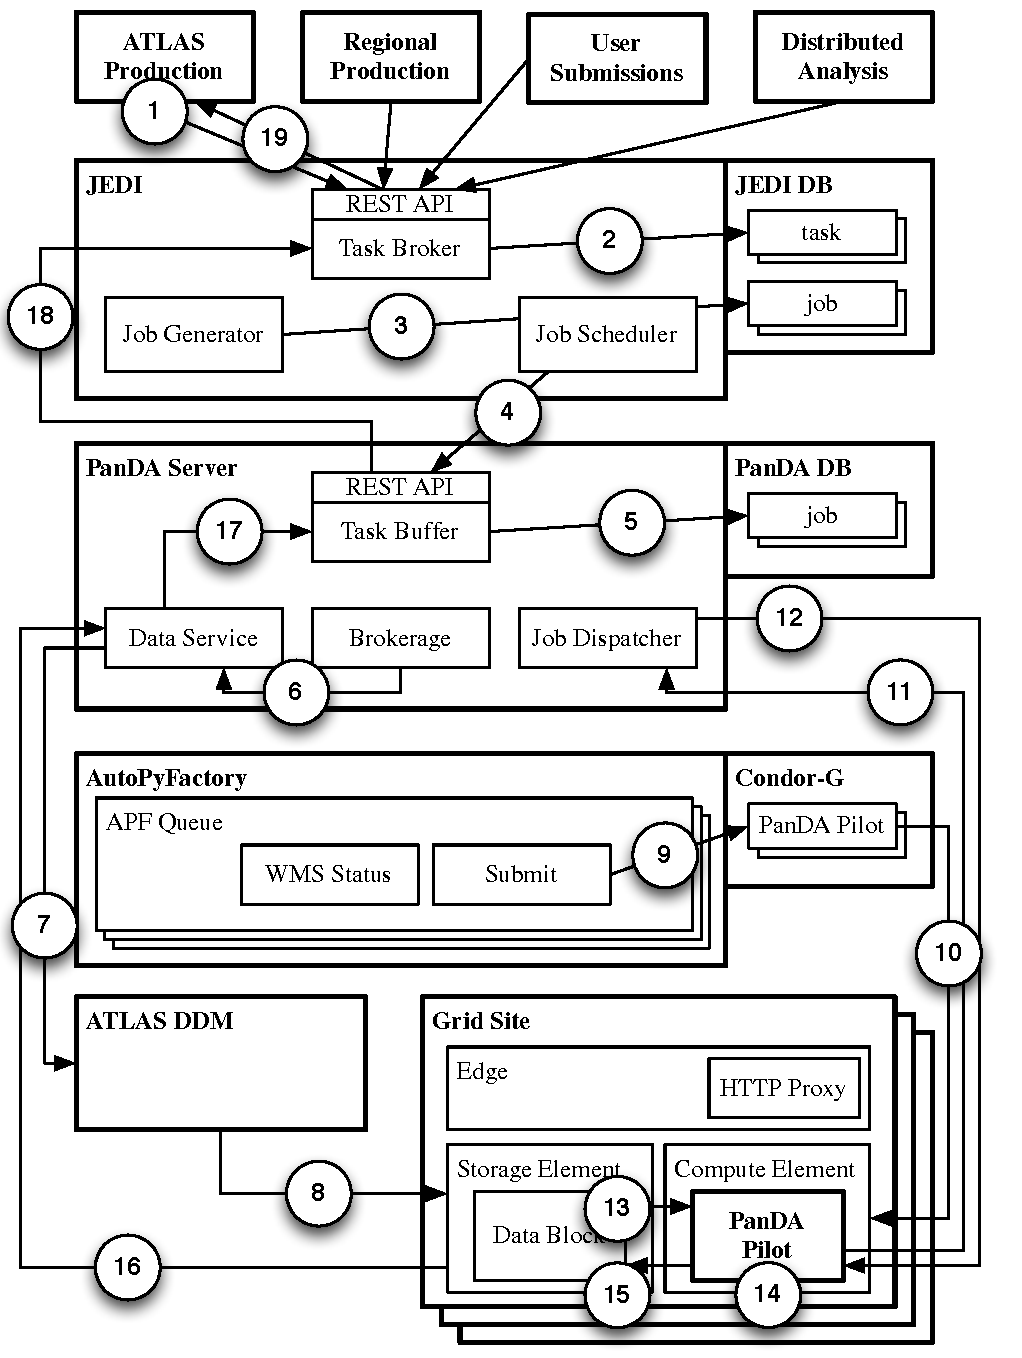
\includegraphics[width=\columnwidth]{figures/panda_architecture.pdf}
  \end{center}
    \caption{PanDA architecture with the subsystems and components
    relevant to the integration of PanDA with supercomputers. Numbers indicates
    the execution process based on JEDI: From the submission of tasks (1) to the
    retrieval of their output (19). The monitoring subsystem, the architectural
    details of PanDA Pilot and the communication among subsystem's components
    are abstracted to improve clarity.}
\label{fig:architecture}
\end{figure}

% -----------------------------------------------------------------------------
% PANDA SERVER
% -----------------------------------------------------------------------------
% \textbf{PanDA Server} is the central hub service of PanDA WMS and it operates
% as a web service~\cite{maeno2011overview}. It consists of four main components
% implemented in Python: Task Buffer, Brokerage, Job Dispatcher, and Data
% Service. Together, these components implement a global queue where to store
% jobs, share information about jobs and their dataset properties with the other
% subsystems, and update their states at execution time.
% -----------------------------------------------------------------------------

% It runs on Apache web server, interacting with the back-end database running
% on separate machines. PanDA Server implements the Apache worker model, with
% many independent processes handling client requests in parallel. Since all
% state is maintained in the central database, the PanDA Server instance itself
% is stateless. Currently, the production version of PanDA utilizes an Oracle
% database as backend, but PanDA Server can also work with the MySQL family of
% databases.

% . It provides a task queue
% managing all job information centrally. The PanDA server receives jobs through
% the client interface into the task queue, upon which a brokerage module
% operates to prioritize and assign work on the basis of job type, priority,
% input data and its locality, and available CPU resources. The PanDA server
%
% and communicating via Python APIs

% Task Buffer manages PanDA's global queue by: (i) storing jobs into the global
% queue; (ii) providing information about and updating the state of each stored
% job. The Brokerage component: (i) matches job attributes with site and pilot
% attributes; (ii) manages the dispatch of input data to processing sites; and
% (iii) derives PanDA's data pre-placement requirement. The Job Dispatcher: (i)
% receives requests from active pilots for new jobs to process; (ii) retrieves
% from Task Buffer the jobs with highest priority and that can be executed on
% the site of the requesting pilot; (iii) creates a wrapper script for the
% selected job, tailored to the site of the requesting pilot; and (iv) monitors
% the state of the job execution on the pilot, updating the Task Buffer
% component. Finally, the Data Service component: (i) retrieves information from
% Task Buffer and Brokerage about the data requirements of each job and the site
% to which each job has been assigned; (ii) interacts with the ATLAS DDM to make
% input files available to the jobs and manage their output data.

% -----------------------------------------------------------------------------
% PANDA PILOT
% -----------------------------------------------------------------------------
% \textbf{PanDA Pilot} implements the execution environment for PanDA's
% jobs\cite{nilsson2011atlas}. Implemented in Python, a PanDA Pilot is launched
% by a wrapper script submitted to a site. Wrapper scripts are tailored to the
% middleware exposed by each site so to maintain PanDA Pilot site-independent.
% PanDA Pilot pulls a job for execution, sets up the execution environment
% including the required input files, spawns the jobs's executable, monitors its
% execution, and supports the output's staging.
% -----------------------------------------------------------------------------

% t: (i) prepares the execution environment for PanDA's jobs, collecting
% information about the compute, data, and network capabilities of the site;
% (ii) requests a job for execution to the Job Dispatcher component of PanDA
% Server; (iii) initiates and monitors the execution of pulled jobs, including
% setting up the job, transferring its input when required, executing the
% payload, transferring output, and checking log files and local space; and (iv)
% cleans up when the payload has finished to execute.

% PanDA is a pilot based workload management system.
% In the PanDA job lifecycle, pilot jobs (Python scripts that organize workload
% processing on a worker node) are submitted to sites. When these pilot jobs
% start on a worker node they contact a central server to retrieve a real
% payload (i.e., an end-user job) and execute it.

% -----------------------------------------------------------------------------
% PILOT DESCRIPTION: COMMENTED OUT BECAUSE WE DESCRIBE IT LATER ON.
% -----------------------------------------------------------------------------
% PanDA Pilot implements the pilot paradigm~\cite{turilli2015comprehensive},
% decoupling resource acquisition from job execution via multi-stage scheduling.
% This has several benefits, including increasing throughput by lowering the
% time taken to queue and schedule jobs; enabling both concurrent and
% sequential job execution depending on the number of cores available to the
% pilot and the time for which it remains available; and exposing a unified and
% consistent interface for the scheduling of jobs, independent from the
% middleware of the site on which the pilot has been instantiated.
% -----------------------------------------------------------------------------

% The specific implementation of PanDA Pilot promotes reliability by
% monitoring the execution of the job's payload, and a certain degree of
% fault-tolerance by recovering information and, possibly, output files from
% jobs that failed, even before instantiating the PanDA Pilot.

% Using these pilot-based workflows helps to improve job reliability, optimize
% resource utilization, allows for opportunistic resources usage, and mitigates
% many of the problems associated with the inhomogeneities found on the Grid.

% Upon bootstrapping, PanDA Pilot downloads major parts of its runtime code via
% HTTP from a central Subversion repository. The repository works with an Apache
% web server, configured with a memory-based web proxy (Squid). The purpose of
% the cache is to reduce the request load on the back-end Subversion server.
% That improves performance since only occasional queries trigger a full lookup
% on the back-end Subversion system, and most external queries are pulled from
% memory on the front-end web server. The benefits of this system include a
% high-performance code download service, combined with code updates still being
% immediately available as soon as they are committed to source code control.

% -----------------------------------------------------------------------------
% AUTOPYFACTORY
% -----------------------------------------------------------------------------
% \textbf{AutoPyFactory} implements a factory to submit pilots locally and to
% both grid and cloud sites~\cite{caballero2012autopyfactory}. Implemented to be
% executed as a single demonized process, AutoPyFactory concurrently spawns
% multiple processes called APFQueue that, on the base of information about jobs
% queued on the PanDA server and on the state and capabilities of resources,
% submit pilots to multiple sites with Condor-G~\cite{frey2002condor}.
% -----------------------------------------------------------------------------

% Each APFQueue communicates with PanDA Server and the Brokerage module to
% collect information about the state of the jobs it manages. On the basis of
% this information, an APFQueue submits new pilots to one site. AutoPyFactory
% implements functionalities to evaluate the number of pilots already
% instantiated on each site, and to apply a consistent and adequate pressure on
% their batch queues. Submission is performed via the Condor-G batch
% system~\cite{frey2002condor}, enabling submission to multiple type of sites.
% AutoPyFactory exposes a dedicated monitoring service, feeding information to
% the PanDA Monitoring subsystem. A proxy manager enables certificate-based
% authentication and authorization for each site.

% As a pilot-based system, PanDA requires some way to get the initial PanDA
% pilot onto worker nodes at sites. This is done with the help of a component
% called AutoPyFactory (APF). APF runs in a single daemonized process,
% launching a separate thread for each internal workflow. Each one of these
% internal workflows typically serves a single job queue as defined in WMS, and
% delivers pilots to a single batch queue, either local or remote. The behavior
% of these APF workflows is determined by the combination of a set of plugins,
% invoked in a fixed order, in a loop, each one in charge of the performance of
% a well defined action.

% -----------------------------------------------------------------------------
% PANDA MONITORING - SPACE SAVING
% -----------------------------------------------------------------------------
% \paragraph{\textbf{PanDA Monitoring}} this subsystem is implemented as a
% web-based, dashboard-style graphical application~\cite{klimentov2011atlas}. It
% runs on Apache and interacts with the back-end database of PanDA Server to
% enable persistence. PanDA Monitoring enables users and site administrators to
% gather information about the status of current and past jobs, data movement,
% and pilot factory. PanDA Monitoring allows users access to all log files of
% each job, greatly simplifying code debugging and failure analysis in a
% distributed computing environment.
% -----------------------------------------------------------------------------

% -----------------------------------------------------------------------------
% JEDI
% -----------------------------------------------------------------------------
% \textbf{JEDI} exposes a task abstraction for workload and workflows
% specification and interfaces with PanDA Server to manage their execution on
% remote sites~\cite{borodin2015scaling}. Implemented as a standalone service,
% JEDI partitions tasks to jobs, and binds these jobs to sites via dedicated
% queues. JEDI collects information about sites' resource capability,
% availability, and performance. Based on this information, JEDI associates
% sites with similar capabilities to a queue. JEDI replaces and extends the
% Brokerage module of the PanDA Server.
% -----------------------------------------------------------------------------

% Each job is assigned to a queue by matching the job's requirements to the
% capability, availability and performance of the sites of that queue. In this
% way,

% This module still handles communication between the Task
% Buffer and the Data Service modules.


% -----------------------------------------------------------------------------
% \subsection{Execution}
% \label{ssec:panda_exec}

% The tasks of workloads and workflows submitted to PanDA are partitioned
% to one or more jobs. Each job is then executed on one of the available
% PanDA Pilots, chosen among those that the PanDA Server manages across multiple
% sites. Tasks processes a certain amount of events that are stored into files,
% and when a task is partitioned to multiple jobs, subsets of events need to be
% assigned to each job and made available to the pilot on which that job will be
% executed. Finally, the output of each job need to be retrieved and aggregated
% into the output of the original task (Fig.~\ref{fig:architecture}).

The relation between tasks and jobs can be one-to-one or one-to-many, and the
conversion between the two can by static or dynamic. During the LHC Run 1, PanDA
required users or applications to perform a static conversion between tasks and
jobs: tasks were described as a set of jobs
% with a fixed number of events
and then submitted to the PanDA Server.

This approach introduced inefficiency both with usability and resource
utilization~\cite{borodin2015unified}. Ideally, users should not have to reason
in terms of jobs: Users conceive analyses in terms of one or more, possibly
related tasks; the `job' abstraction is required by the execution middleware,
i.e. PanDA. Further, a static partitioning of tasks into jobs does not take into
account the heterogeneity and dynamicity of the resources of the pilots on which
each job will be executed.

Another problem of static job sizing is that PanDA instantiates pilots on sites
with different type of resources and different models of availability of those
resources. An optimal sizing of each job should take into account these
properties. For example, sites may offer cores with different speed, networking
with different amount of bandwidth, and resources could be guaranteed to be
available for a defined amount of time or could disappear at any point in time
as with opportunistic models of resource provision.

JEDI was deployed for the LHC Run 2 to address these inefficiencies. Users or
the application layer submits tasks descriptions to JEDI
(Fig.~\ref{fig:architecture}:1) that stores them into a queue implemented by a
database (Fig.~\ref{fig:architecture}:2). Tasks are partitioned into jobs of
different size, depending on both static and dynamic information about available
resources (Fig.~\ref{fig:architecture}:3). Jobs are bound to sites with
resources that best match jobs' requirements, and submitted to the PanDA Server
for execution (Fig.~\ref{fig:architecture}:4).

Once submitted to the PanDA Server, jobs are stored by the Task Buffer component
into a global queue implemented as a  database (Fig.~\ref{fig:architecture}:5).
When jobs are submitted directly to the PanDA Server, the Brokerage component is
used to bind jobs to available sites, depending on static information about the
resources available for each site. Jobs submitted by JEDI are already bound to
sites so no further brokerage is needed.

Once jobs are bound to sites, the Brokerage module communicates to the Data
Service module what data sets need to be made available on what site
(Fig.~\ref{fig:architecture}:6). The Data Service communicates these
requirements to the ATLAS DDM (Fig.~\ref{fig:architecture}:7) that, when needed,
takes care of % aggregating files into datasets and containers,
replicating them on the required sites (Fig.~\ref{fig:architecture}:8).

% AutoPyFactory subsystem communicates with the Task Buffer component of the
% PanDA Server, acquiring information about jobs that are ready for execution on
% specific (type of) sites (Fig.~\ref{fig:architecture}:9). On the basis of this
% information,
Meanwhile, AutoPyFactory defines a set of suitable PanDA Pilots and concurrently
submits them to a Condor-G broker (Fig.~\ref{fig:architecture}:9). This broker
submits these pilots wrapped as jobs or VMs to the required sites
(Fig.~\ref{fig:architecture}:10).

% AutoPyFactory submits pilots only when similar pilots are not yet available
% and maintains a predefined amount of pressure on the queue of each site. In
% this way, resource availability and utilizations is optimized.

When a PanDA Pilot becomes available on a site, it calls the Job Dispatcher
module of the PanDA Server, requesting for a job to execute
(Fig.~\ref{fig:architecture}:11). The Job Dispatcher interrogates the Task
Buffer module for a job that is bound to the site of that pilot and ready to be
executed. Task Buffer checks the global queue (i.e., the PanDA database) and,
upon availability, returns a suitable job the Job Dispatcher. The Job Dispatcher
dispatches that job to the PanDA Pilot (Fig.~\ref{fig:architecture}:12).

% \mtnote{Can a pilot request multiple jobs to execute
% concurrently?}\sergeynote{In principle it should be able to do that, but
% that's not how it is operated. One pilot - one job is a cleaner model in an
% environment where resources are ``owned'' by the organization that runs
% pilots. Simplifies many things. At least as far as I know.}

Upon receiving a job, a PanDA Pilot starts a monitoring process and forks a
subprocess for the execution of the job's payload. The job is set up, input data
are transferred from the designated staging-in location
(Fig.~\ref{fig:architecture}:13), and the job's payload is executed
(Fig.~\ref{fig:architecture}:14). Once completed, output is transferred to the
staging-out location (Fig.~\ref{fig:architecture}:15).

% During the job's payload execution, the monitoring process of PanDA Pilot
% checks the status of the job execution and its environment.

The Data Service module of the PanDA Server tracks and collects the output
generated by each job (Fig.~\ref{fig:architecture}:16), updating jobs'
attributes via the Task Buffer module (Fig.~\ref{fig:architecture}:17). When the
output of all the jobs of a task are retrieved, it is made available to the user
via PanDA Server. When a task is submitted to JEDI, task is instead marked as
done (Fig.~\ref{fig:architecture}:18) and the result of its execution is made
available to the user by JEDI (Fig.~\ref{fig:architecture}:19).

% \mtnote{Think whether a comparison with other WMS based on the review we did
% makes sense in this context.}\sergeynote{You provided a nice description of
% the PanDA system here.}



% ----------------------------------------------------------------------------
% IV - DEPLOYING PANDA ON A LEADERSHIP-SCALE SYSTEM
% ----------------------------------------------------------------------------
\section{Deploying PanDA on a Leadership-scale system}
\label{sec:panda_deployment}

\begin{enumerate}
  \item Why? To support a specific stage of the ATLAS Monte Carlo Workflow.
  \item Challenges
  \item Opportunities
  \item Highlight distinction of PanDA on wide-area distributed systems vs on TITAN
  \item Take-aways, lessons learned
\end{enumerate}

\subsection{OLCF and Titan}

In 2004, the Oak Ridge Leadership Computing Facility (OLCF) was established at
Oak Ridge National Laboratory (ORNL). The OLCF's mission is to accelerate
scientific discovery and engineering progress by providing outstanding computing
and data management resources to high-priority research and development
projects. Among other resources, OLCF manages Titan, a leadership-class and the
fastest open-science supercomputer in the US. Titan enables scientists to
evaluate and assess various complex physical phenomena via large-scale
computational simulations.

Titan is a Cray XK7 system with 18,688 compute nodes~\cite{top500}. Each compute
node is equipped with an AMD Opteron CPU and a Nvidia Tesla GPU. This hybrid
design provides improved energy efficiency, as well as an order of magnitude in
computational capacity over its predecessor. Titan has 710 TB of total system
memory and a center-wide parallel file system known as Spider II~\cite{spider2}.
Spider II is one of the world's fastest and largest POSIX complaint parallel
file systems, designed to serve write-heavy I/O workloads generated by Titan
compute clients and other OLCF resources.


% The topology and architecture details of Spider II infrastructure are
% illustrated in Figure~\ref{fig:xk7-compute-node} and
% described as follows:
%
%
% \begin{figure}[!htb]
%     \centering
%     \begin{tabular}{cc}
%         {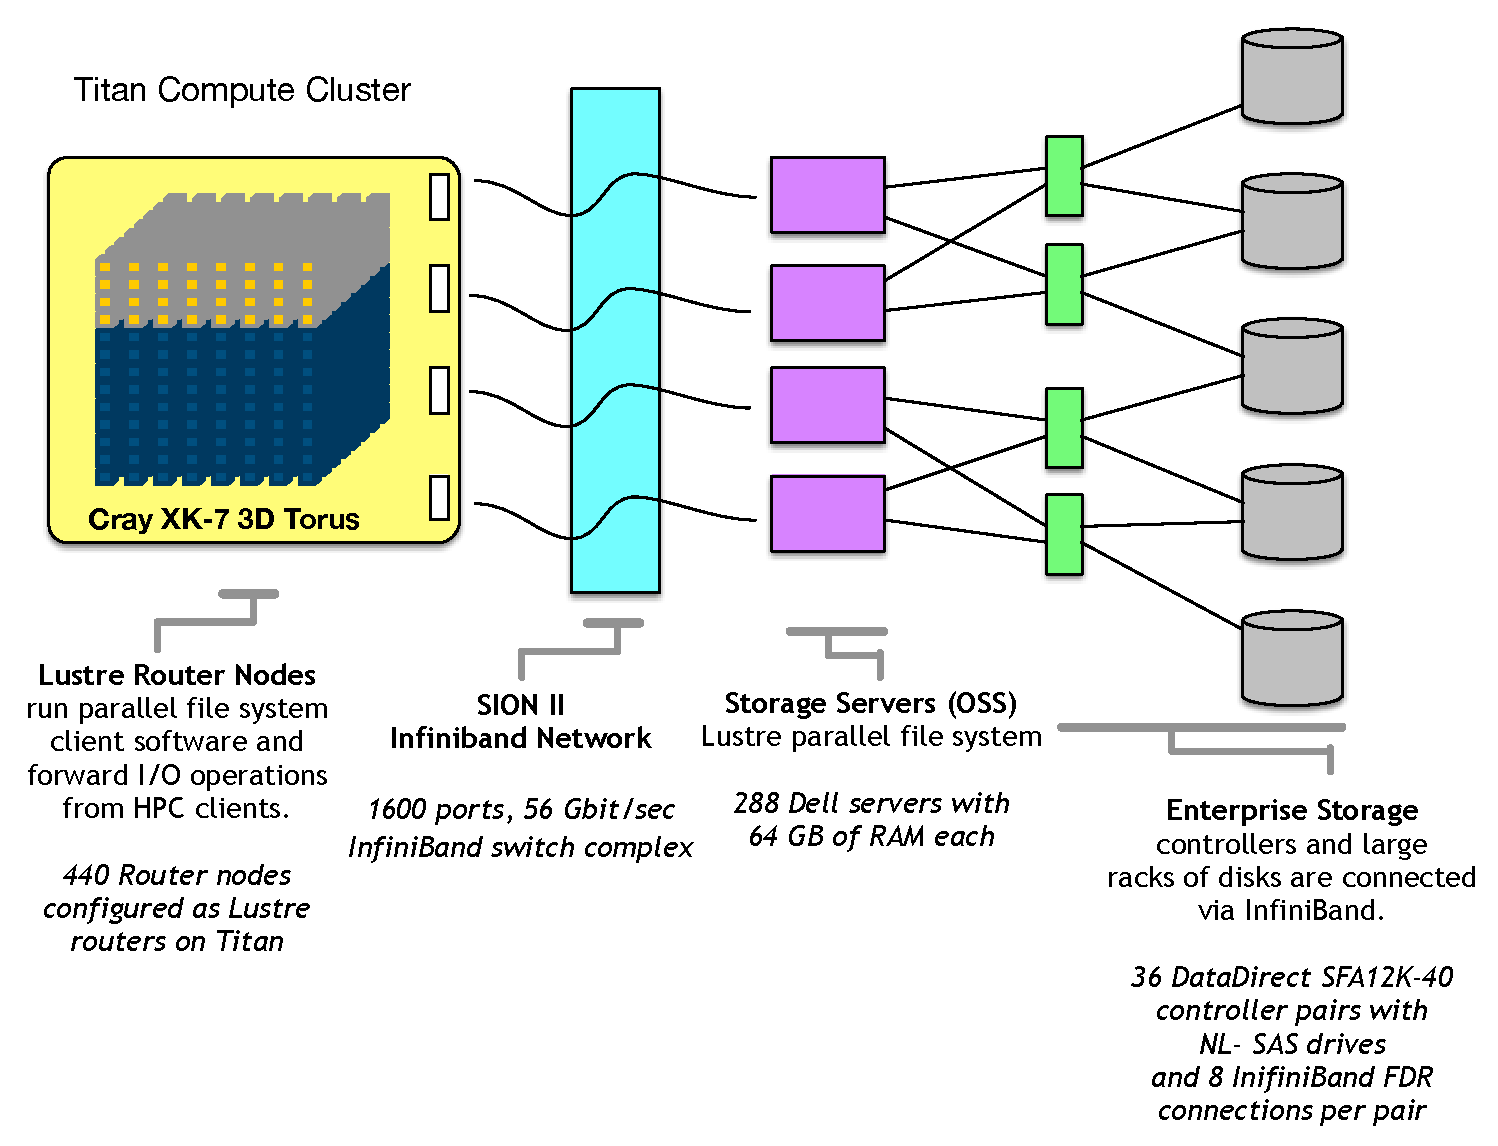
\includegraphics[width=0.48\textwidth]{figures/spider2arch.pdf}}\\
%     \end{tabular}
%     \caption{Infrastructure and I/O path between Titan (Cray XK7) and its backend storage}
%     \label{fig:xk7-compute-node}
% \end{figure}
%
%
%
% Spider II is based on the Lustre technology~\cite{lustre}.  It is configured
% and deployed as two independent, non-overlapping file systems, each with 144
% Lustre Object Storage Servers (OSSs) and 1,008 Lustre Object Storage Targets
% (OSTs). Spider II offers ~30 PB usable file system capacity to OLCF systems and
% users and has over 1 TB/s aggregate write I/O performance.

The next LHC run for taking data (Run 3) will require more resources than the
Worldwide LHC Computing Grid (WLCG) can provide. Currently, PanDA WMS uses more
than 100,000 cores at over 100 Grid sites, with a peak performance of 0.3
petaFLOPS. This capacity will be sufficient for the planned analysis and data
processing, but it will be insufficient for the Monte Carlo production workflow
and any extra activity. To alleviate these challenges, ATLAS is engaged in a
program to expand the current computing model to include additional resources
such as the opportunistic use of supercomputers as well as commercial and
academic clouds.


% -----------------------------------------------------------------------------
\subsection{Use of Supercomputers with PanDA}
\label{ssec:panda-supercomputers}

Modern supercomputers have been designed mainly to support parallel computation
that requires runtime communication. Job execution is parallelized across
multiple cores, each core calculating a small part of the problem and
communicating with other cores via a message passing interface (MPI).
Accordingly, supercomputers have large number of worker nodes, connected through
a high-speed, low-latency dedicated network. Each worker node has multicore
CPUs, usually augmented with parallel Graphics Processing Units (GPUs) or other
types of specialized coprocessors.

% \sergeynote{specifically "distributed Grid computing"}\mtnote{done.}.
% \sergeynote{geographically distributed?}\mtnote{Better?}

PanDA WMS has been designed to support distributed Grid computing. Executing
ATLAS workloads or workflows involves concurrent and/or sequential runs of
possibly large amount of jobs, each requiring no or minimal parallelization and
no runtime communication. Thus, computing infrastructure like WLCG have been
designed to aggregate large amount of computing resources across multiple sites.
While each site may deploy runtime message-passing capabilities, usually these
are not used to perform distributed computations.

There are at least two approaches to enable PanDA WMS to execute ATLAS workloads
or workflows on supercomputers: (i) using the subset of resources and
capabilities shared by both supercomputers and WLCG; (ii) reconciling the
parallel and distributed computing paradigms by means of dedicated abstractions.
The former is a pragmatic approach that enables the execution of specific
workloads by prototyping single-point solutions. The latter is a principled
approach, better suited for a production-grade solution, capable of supporting
general-purpose workloads and workflows on both supercomputers and Grid
infrastructures. These two approaches are not mutually exclusive: developing a
single-point solution gives the opportunity to better understand the problem
space, supporting the creation of abstractions for the integration of computing
paradigms.

This section illustrates the design and architecture of a job broker prototyped
by the PanDA team. This broker supports execution of part of the ATLAS
production Monte Carlo workflow on Titan, a leadership-class supercomputer
managed by the Oak Ridge Leadership Computing Facility (OLCF) at the Oak Ridge
National Laboratory (ORNL). After an analysis of the results obtained and the
lessons learned, the following section introduces the design and first
experimental characterization of a next generation executor (NGE). NGE is
designed to abstract resources and capabilities, enabling the concurrent
execution of both parallel and distributed computing on generic high performance
computing (HPC) machines.


% -----------------------------------------------------------------------------
\subsection{Interfacing PanDA with Titan}
\label{ssec:panda-titan}

The Titan supercomputer, current number three on the Top 500 list~\cite{top500},
is a Cray XK7 system with 18,688 worker nodes and a total of 299,008 CPU cores.
Each worker node has an AMD Opteron  6274 16-core CPU, a Nvidia Tesla K20X GPU,
32 GB of RAM and no local storage, though a 16 GB RAM disk can be set up. Work
nodes use Cray’s Gemini interconnect for inter-node MPI messaging. Titan is
served by the Spider II~\cite{spider2}, a Lustre filesystem with 32 PB of disk
storage, and by a 29 PB HPSS tape storage system. Titan’s worker nodes run
Compute Node Linux, a run time environment based on SUSE Linux Enterprise
Server.

% Titan, was the first large-scale system to use a hybrid architecture that
% utilizes worker nodes with both AMD 16-core Opteron 6274 CPUs and NVIDIA Tesla
% K20 GPU accelerators. This hybrid design provides improved energy efficiency,
% as well as an order of magnitude in computational capacity over its
% predecessor.

Titan's users submit jobs to Titan's PBS scheduler by logging into login or data
transfer nodes (DTNs). Titan's authentication and authorization model is based
on two-factor authentication with a RSA SecurID key, generated every 30 seconds.
Login nodes and DTNs have out/inbound wide area network connectivity while
worker nodes have only local network access. Fair-share and allocation policies
are in place both for the PBS batch system and shared file systems.

% Data staging is supported via the DTNs, from the wide area network and from
% the OLCF high performance storage system (HPSS). DTNs are shared across all
% Titan's users that can schedule jobs to a dedicates batch system to automate
% data staging. Fair-share policies are in place both for the batch system and
 %for the use of DTN resources.

Titan's architecture, configuration and policies poses several challenges to the
integration with PanDA. The deployment model of PanDA Pilot is unfeasible on
Titan: PanDA Pilot requires to contact the Job Dispatcher of the PanDA Server to
pull jobs to execute but this is not possible on Titan because worker nodes do
not offer outbound network connectivity. Further, Titan does not support PanDA's
security model based on certificates and virtual organizations, making the
PanDA's approach to identity management also unfeasible. While DTNs offer wide
area network data transfer, an integration with ATLAS DDM is beyond the
functional and administrative scope of the current prototyping phase. Finally,
the specific characteristics of the execution environment, especially the
absence of local storage on the worker nodes and modules tailored to Compute
Node Linux, require reengineering of ATLAS application frameworks.

Currently, no HEP application can benefit from Titan's GPUs but some
computationally-intensive and non memory-intensive tasks can be offloaded from
the Grid to Titan's large amount of cores. Further, when HEP tasks can be
partitioned to independent jobs, Titan worker nodes can be used to execute up to
16 concurrent jobs' payload, one for each available core. Given these
constraints and challenges, the type of task most suitable for execution at the
moment on Titan is Monte Carlo
% event generation and
detector simulation.
% Both types of task are
This type of task is mostly computational-intensive, requiring less than 2GB of
RAM at runtime and with small input data requirements. Detector simulation tasks
in ATLAS account for XX--XX\% of all jobs on WLCG, corresponding to X/X of the
current Grid capacity.\mtnote{Please provide numbers to replace `XX' and,
possibly, a diagram illustrating detector simulation stats compared to the whole
ATLAS computation activity.}

Detector simulation is part of the ATLAS production Monte Carlo (MC) workflow
(also known as MC production
chain)~\cite{rimoldi2006atlas,de2013delphes,ritsch2014atlas}. The MC workflow
consists of four main stages: event generation, detector simulation,
digitization, and reconstruction. Event generation creates sets of particle
four-momenta via different generators, e.g., PYTHIA~\cite{sjostrand2006pythia}
and HERWIG~\cite{corcella2001herwig}. The detector simulator is called
Geant4~\cite{agostinelli2003geant4} and simulates the interaction of these
particles with the sensitive material of the ATLAS detector. Each interaction
creates a so-called hit and all hits are collected and passed on for
digitalization where hits are further process to mimic the readout of the
detector. Finally, reconstruction operates local pattern recognition, creating
high-level objects like particles and jets.

% While this is different from the HEP computing paradigm, where jobs are
% independent, it still shares common features such as the use of
% parallelization. It is not a requirement that HPC machines are able to run
% any possible task, nor is it relevant how many kinds of job types that can be
% run. What matters is the total number of cycles that can be offloaded from
% the Grid.

% Standard ATLAS workflow can not be easily ported to supercomputers due to
% several complications such as specialized worker node setups, no outbound
% network connections, limited memory per node, custom operating systems, etc. A
% reorganization of the standard workflow is therefore needed.

% -----------------------------------------------------------------------------
\subsection{PanDA Broker on Titan}
\label{ssec:panda_titan}

The lack of wide area network connectivity on Titan's worker nodes is the most
relevant challenge for integrating PanDA WMS and Titan. Without connectivity,
Panda Pilots cannot be scheduled on worker nodes because they would not be able
to communicate with PanDA Server and therefore pull and execute jobs. This makes
impossible to port PanDA Pilot to Titan while maintaining the defining feature
of the pilot abstraction: decoupling resource acquisition from workload
execution via multi-stage scheduling.

The unavailability of pilots is a potential drawback when executing distributed
workloads like MC detector simulation. Pilots are used to increase the
throughput of distributed workloads: while pilots have to wait in the
supercomputer's queue, once scheduled, they can pull and execute jobs
independently from the system's queue. Jobs can be concurrently executed on
every core available to the pilot, and multiple generations of concurrent
executions can be performed until the pilot's walltime is exhausted. This is
particularly relevant for machines like Titan where queue policies privilege
parallel jobs on the base of the number of worker nodes they request: the higher
the number of nodes, the shorter the amount of queue time (modulo fair-share and
allocation policies).

% MC event generation and simulation tasks can be executed without pilots but
% the time spent waiting in the queue would be too large compared to the
% execution time of each task.

Titan’s backfill functionality offers the opportunity to avoid the overhead of
queue wait times without using pilot abstraction. Backfill availability is the
number of worker nodes that cannot be used for a certain amount of time by any
of the jobs already queued on Titan: All queued jobs are either too large or
their walltime is too long. At any point in time, Titan’s Moab scheduler can be
queried for backfill availability. Based upon the result of this query, a job
can be shaped to request no more than the backfill availability. As such, when
submitted this job is usually scheduled immediately, spending almost no time in
the queue.

Compared to pilots, backfill has the disadvantage of limiting the amount of work
nodes that can be requested. Pilots are normal jobs: they can request as many
worker nodes for as much time as a queue can offer. On the contrary, jobs sized
on the basis of backfill information availability \jhanote{should be resource
availability or backfill queue information?}\mtnote{AFAIH, there is no dedicated
queue to backfill} depend on the number of worker nodes that cannot be given to
any other job in the Titan's queue.
% \sergeynote{any other job currently in the Titan's queue?}\mtnote{Better?}.

Usually, backfill availability is a fraction of the total capacity of the queue
but the size of Titan mitigates this limitation. Every year, about 10\% of
Titan's capacity remains unused, corresponding to an average of 30,000 unused
cores. This equals approximately 270M core hours per year, roughly 30\% of the
overall capacity of WLCG.

% A system that can use those temporarily free worker nodes with smaller
% scale tasks would be very valuable. For this reason, Titan offers backfill
% functionalities: users can interrogate Titan's Moab scheduler about how many
% free nodes are currently available and for how long. If a user submit a
% requestvfor that number of nodes and walltime, queue time will be minimal.

\mtnote{Please feel free to add details about backfill as needed.}
\mtnote{Please note: I know the following departs for the current name given to
the PanDA subsystem installed on Titan. I think there is a good reason to call
it a broker instead of a pilot, and I think I explained it in the previous
paragraphs. Please  take this just as a suggestion, something I would like to
discuss in our meeting.} \sergeynote{It's not a pilot in conventional sense. I
call it an agent. It just happened that we were able to use full PanDA pilot's
code base to serve our purposes on Titan. that's why, by inertia, we still call
it a pilot.}\mtnote{Thank you. We would have a problem calling it `agent' as we
use that term to name the pilot of NGE. Would PanDA Broker work?}\mtnote{Sergey
agreed that we should not use `pilot'. He is quite convinced by `broker' but we
are both open to better suggestions.}

Given the communication requirements of PanDA Pilots and the unused capacity of
Titan, PanDA pilot was redesigned to serve as a job broker on Titan. Architected
as a stand-alone service to be executed on a DTN, this prototype called `PanDA
Broker' implements functionalities to: (i) interrogate Titan about backfill
availability; (ii) pull MC jobs and events; (iii) wrap the payload of ATLAS jobs
into MPI scripts; (iv) submitting MPI scripts to Titan's PBS batch system and
monitor their execution; and (v) staging input/output files. Backfill querying,
payload wrapping, and scripts submission required a new implementation while
pulling ATLAS job and events, and file staging were mostly inherited from PanDA
Pilot.

% \sergeynote{Monitor job state and state transitions using
% SAGA}\mtnote{Better?}

\begin{figure}
  \begin{center}
    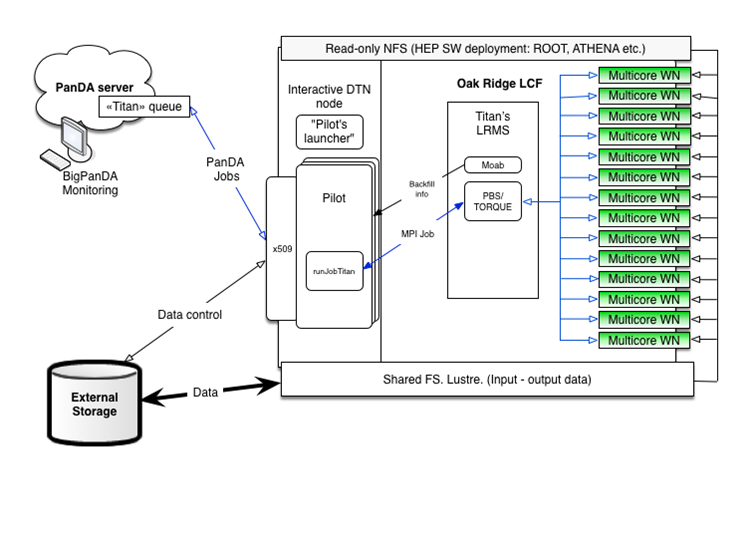
\includegraphics[width=\columnwidth]{figures/PanDA_setup_at_OLCF.png}
    \caption{Schematic view of the PanDA Broker.}
  \end{center}
\label{fig:panda_broker}
\end{figure}

Backfill querying is performed via a dedicated Moab scheduler command while a
tailored Python MPI script is used to execute the payload of ATLAS jobs. This
MPI script enables the execution of unmodified Grid-centric, ATLAS jobs on
Titan. Typically, a MPI script is workload-specific as it sets up the execution
environment for a specific payload. This involves organization of worker
directories, data management, optional input parameters modification, and
cleanup on exit. Upon submission, a copy of the MPI script runs on every
available worker node,
% Each script knows its MPI rank (an index that runs from zero to a maximum
% number of nodes or script copies) as well as the total number of ranks in the
% current submission. When activated on worker nodes, each copy of the MPI
% script
starting the execution of the ATLAS job's payload in a subprocess and waits
until its completion.

MPI scripts are submitted to Titan's PBS batch system via
RADICAL-SAGA~\cite{radical-saga_url}, a Python module, compliant with the OGF
GFD.90 SAGA specification~\cite{goodale2008simple}. The Simple API for Grid
Applications (SAGA) offers a unified interface to diverse job schedulers and
file transferring services. In this way, SAGA provides an interoperability layer
that lowers the complexity of using distributed infrastructures. Behind the API
façade, RADICAL-SAGA implements a adaptor architecture: each adaptor interface
the SAGA API with different middleware systems and services, including the PBS
batch scheduler of Titan.

The data staging capabilities of the PanDA Broker are implemented via a file
system that is shared among DTNs and worker nodes. The input files with the
events of the ATLAS jobs are downloaded on the shared filesystem via the ATLAS
DDM service. The MPI script setup process includes making the location of these
files available to the payload of the ATLAS's jobs. The PanDA Broker can locate
the payload's output files on the shared filesystem and transfer them from Titan
to any computing center used by ATLAS.
% the ATLAS Tier 1 computing center at Brookhaven National Lab (BNL) or any
% other Grid site.

Once deployed on Titan, every PanDA Broker supports the execution of MC detector
simulation in 8 steps: (i) PanDA Broker queries Titan's Moab scheduler about
current backfill availability; (ii) the PanDA Broker queries the Job Dispatcher
module of the PanDA server for ATLAS jobs that have been bound to Titan by JEDI;
(iii) the PanDA Broker requests to the Data Service module of the PanDA Server
what input data these ATLAS jobs require and transfer the files to the DTN via
the ATLAS DDM service; (iv) the PanDA Broker creates an MPI script, wrapping
enough ATLAS jobs' payload to fit backfill availability; (v) the PanDA Broker
submits the MPI script to the Titan's PBS batch system via RADICAL-SAGA; (vi)
upon execution on the worker node(s), the MPI script creates a ramdisk and
configure AthenaMP to execute the ATLAS jobs' payload; (vii) the payload is
executed into dedicated processes, 16 for each worker node, 1 for each available
core; (viii) upon completion of the payload execution, the PanDA Broker locates
the output on the shared filesystem and transfer it to designated computing
centre.

% from the Job Dispatcher module of PanDA Server (as done by a PanDA Pilot);
% (iii) downloading events via PanDA Server's Data Service from ATLAS DDM to
% Titan's DTN; (iv) wrap the Geant4 payload into a PBS job; (v) submit jobs to
% Titan's PBS batch scheduler;

% Integration with Titan is the current focus for PanDA developers.

% The project aims to integrate Titan with the PanDA system using an updated
% PanDA Pilot that runs on the front-end node and submits ATLAS payloads to the
% worker nodes using the local batch system (PBS) via the SAGA (Simple API for
% Grid Applications) interface~\cite{SAGA}. This solves several complications
% of running on HPC worker nodes, including the lack of connectivity to outside
% world. The pilot can communicate with the PanDA server from the front-end
% machine.

% \paragraph*{HPC Backfill} HPC facilities are geared towards large scale jobs
% by design. Time allocation on an HPC is competitive and large projects are
% often preferred. About 10\% of capacity on a typical HPC machine is unused
% due to mismatches between job sizes and available resources. The worker nodes
% sit idle because there are not enough of them or they do not have enough time
% to handle a large scale computing job. On a machine of the scale of Titan,
% these 10\% correspond to estimated 300M core hours per year. A system that
% can occupy those temporarily free nodes with smaller scale tasks would be
% very valuable.

% This offers a great possibility for PanDA to harvest the opportunistic
% resources on Titan and use a similar mechanism on other HPCs. Functionality
% has been added to the PanDA Pilot to collect information about available
% unused worker nodes on Titan in real time.

% First test of the system were quite successful and show great promise in
% increasing the resource utilization on Titan.



% ----------------------------------------------------------------------------
% VI - PERFORMANCE CHARACTERIZATION
% ----------------------------------------------------------------------------
\section{Performance Characterization}
\label{sec:panda_titan}

Currently, ATLAS deploys 20 instances of the PanDA Broker on 4 Titan's DTNs, 5
instances per DTN. Each broker submits and manages the execution of 15 to 300
ATLAS jobs, one job for each worker node, and a theoretical maximum concurrent
use of 96,000 cores. Since November 2015, PanDA Brokers have operated only in
backfill mode, without a defined time allocation, and running at the lowest
priority on Titan.

We evaluate the efficiency, scalability and reliability of the deployment of
PanDA WMS on Titan by characterizing the behavior of both PanDA Broker and
AthenaMP. All the measurements were performed between January 2016 and February
2017, hereafter called `experiment time window'.

% two dimensions: (i) backfill utilization by the PanDA Brokers; and (ii) the
% amount of runtime spent performing detector simulations.

% We based our characterizations on measuring the number of cores utilized by
% ATLAS on Titan, the overall backfill availability, the number of detector
% simulations performed on all the resources available to ATLAS and on Titan,
% and the failure rate of these simulations. We also consider the the time taken
% to setup AthenaMP and to simulate events in the ATLAS detector with it. All
% the measurements were performed between January 2016 and February 2017,
% hereafter called `experiment time window'.

% \mtnote{TODO: expand the previous paragraph to include dimensions of AthenaMP
% characterization.}

% -----------------------------------------------------------------------------
\subsection{Characterizing the PanDA Broker on Titan}
\label{ssec:broker_titan}

% Figure~\ref{fig:backfill-utilization} (gray bars) shows the number of
% core-hours used by ATLAS during the experiment time window. ATLAS consumed a
% total of 73.8M core-hours, for an average of $\approx$7M core-hours a month,
% with a minimum of 3.3M core-hours in April 2016 and a maximum 14.8M core-hours
% in February 2017.

We calculate the total amount of backfill availability over a period of time by:
(i) polling the available backfill slots at regular intervals during that time
window; (ii) converting the number of worker nodes available and their walltime
into core-hours; (iii) summing the number of core-hours. We call this number of
core-hours `total backfill availability'.

Figure~\ref{fig:backfill-utilization} shows the total backfill availability on
Titan (gray bars) and the number of core-hours of that availability used by
ATLAS (blue bars) during the experiment time window. ATLAS consumed a total of
51.4M core-hours, for an average of $\approx$3.7M core-hours a month, with a
minimum of 1.7M core-hours in April 2016 and a maximum 7.9M core-hours in
February 2017.

\begin{figure}[htp]
    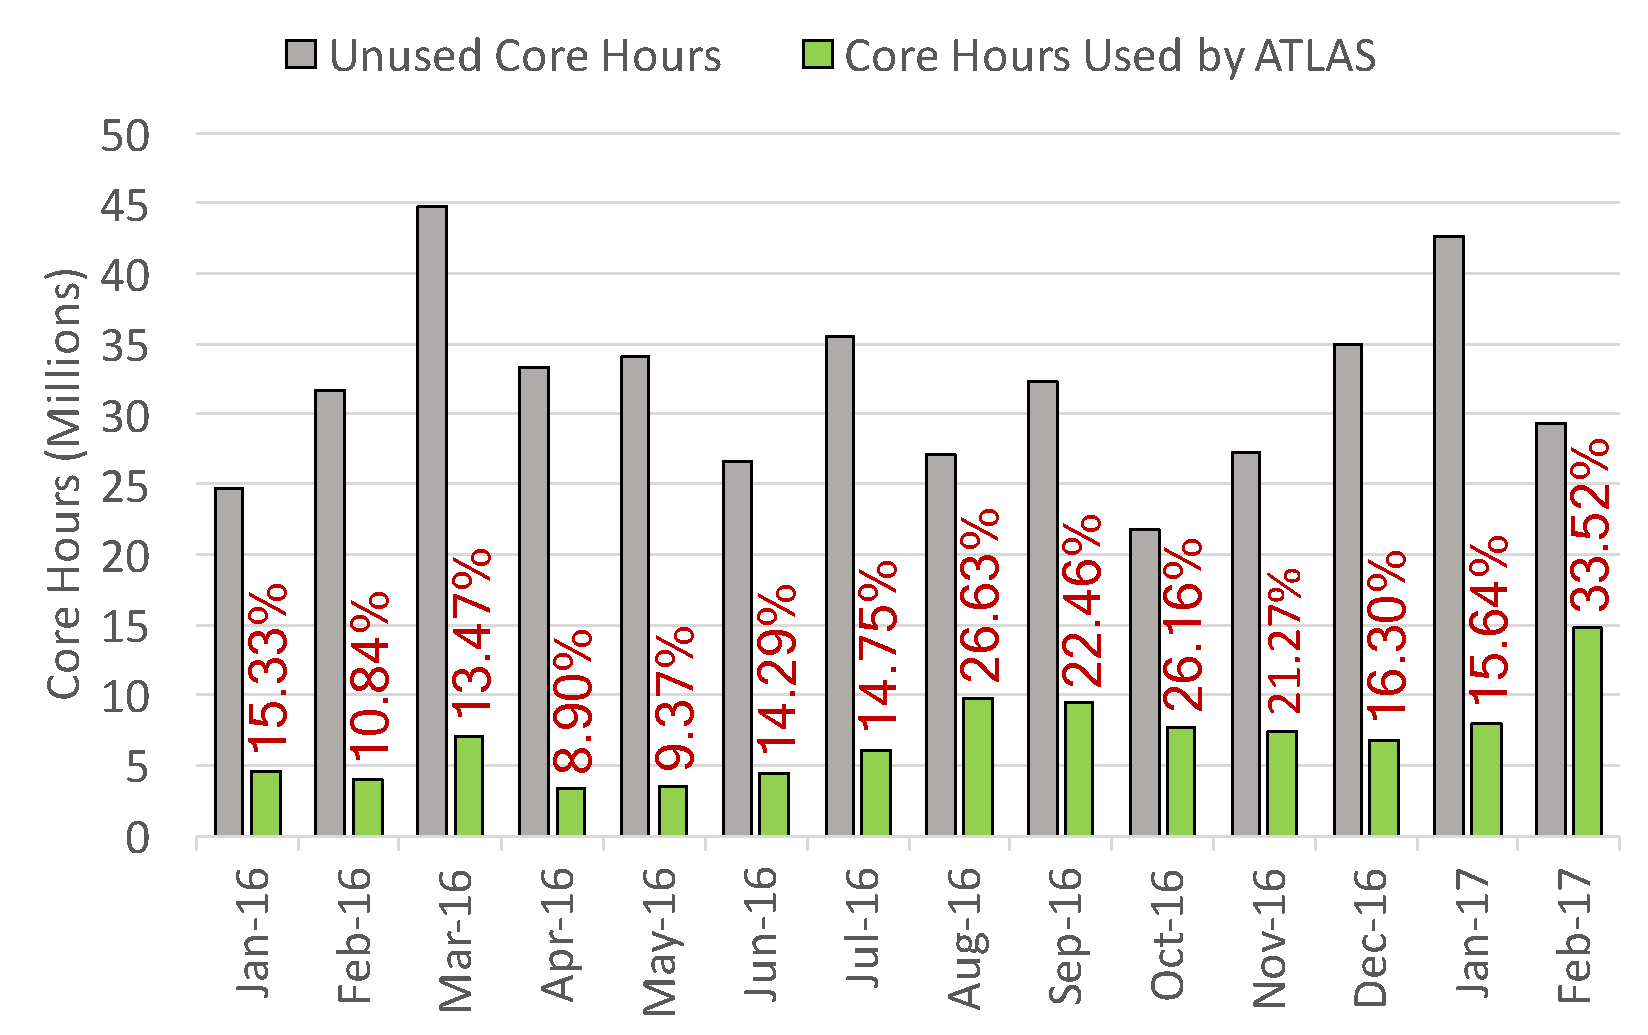
\includegraphics[clip,width=\columnwidth]{figures/backfill_consumption.pdf}

    \caption{Titan's total backfill availability: CPU core-hours (gray) and CPU
    core-hours used by ATLAS (blue). GPU core-hours unaccounted for as they
    cannot be used by ATLAS. Efficiency of PanDA Brokers defined as percentage
    of total Titan's backfill availability used by ATLAS (Red labels).}

\label{fig:backfill-utilization}
\end{figure}

PanDA Brokers' efficiency (Figure~\ref{fig:backfill-utilization}, red labels) is
defined as the fraction of core-hours utilized by the PanDA Brokers to  Titan’s
total backfill availability during the experiment time window. The brokers
reached 18\% average efficiency, with a minimum 7.8\% efficiency on May 2016 and
a maximum 30.9\% efficiency on February 2017.
% The total backfill available was 38.1M Titan core-hours in April 2016, and
% 33.1M Titan core-hours in February 2017. This shows that the measured
% difference in efficiency did not depend on a comparable difference in total
% backfill availability.
The total backfill availability was 20.3M in April 2016, and 17.6M in February
2017. This shows that the measured difference in efficiency did not depend on a
comparable difference in the total backfill availability.

% \mtnote{Elaborate further and put it at the end, after giving several of the
% measurements we would need. ``Currently, this measure of efficiency is being
% refined on the base of the actual minimum amount of walltime that PanDA Broker
% can request when submitting job requests. This is not a fixed value as it
% depends on variable initialization and configuration overheads, simulation
% time, and number of nodes obtained. Part of the undergoing effort is to
% enable the measurements of  the distribution of these parameters to derive an
% optimization function.''}

% \jhanote{I would plot the efficiency on the Y2 axis for both
% [diagrams].}\mtnote{Done but then the first diagram ended up plotting a subset
% of the data of the second diagram. I used only the second diagram.} \jhanote{I
% would suggest similar style of X-axis as previous figure. Difficult to parse
% which is April if we are going to call out a specific month. Also consistency
% in style is generally good to keep cognitive burden low.}\mtnote{Done.}

% Figure~\ref{fig:hpc-workload-utilization} shows that d

During the experiment time window, about 2.25M detector simulation jobs were
completed on Titan, for a total of 225M events processed. This is equivalent to
0.9\% of all the 250M detector simulations performed by ATLAS in the same period
of time, and 3.5\% of the 6.6B events processed by those jobs.
% Comparatively, Titan contributed 3.9\% of the total of around
% 200K\mtnote{TODO: Fix this number} cores available to ATLAS on Grid, Cloud,
% and HPC infrastructures together.
These figures confirms the relevance of supercomputers' resource contribution to
the LHC Run 2, especially when accounting for the amount of unused total
backfill availability and the improvement of PanDA efficiency across the
experiment time window.

% \begin{figure}[htp]
%     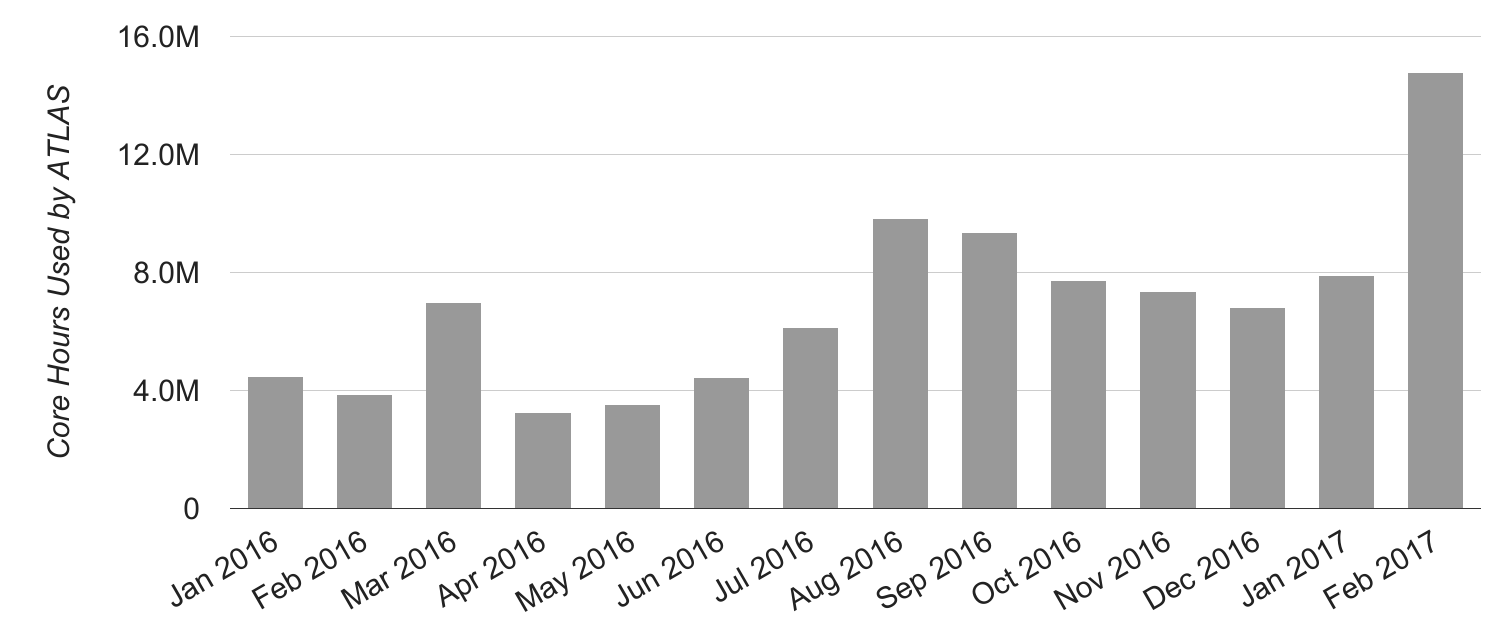
\includegraphics[clip,width=\columnwidth]{figures/cpu_hours.png}
% \caption{\mtnote{Placeholder for the diagram/data I asked to Danila and
% Sergey. Consider a table instead of a figure.}}
% \label{fig:hpc-workload-utilization}
% \end{figure}

On February 2017, PanDA Brokers used almost twice as much total backfill
availability than in any other month (preliminary results for March 2017
displayed in Fig.~\ref{fig:backfill-utilization} confirm this trend). No
relevant code update was made during that period and logs indicated that the
brokers were able to perform faster. This is likely due to hardware upgrades on
the DTNs. The absence of continuous monitoring of those nodes does not allow to
quantify bottlenecks but spot measurements of their load indicate that a faster
CPU and better networking were likely responsible for the improved performance.
Investigations showed an average CPU load of 3.6\% on the upgraded DTNs. As
such, further hardware upgrades seem unlikely to improve significantly the
performance of PanDA Brokers.

Every detector simulation executed on Titan process 100 events. This number of
events is consistent with the physics of the use case and with the average
duration of backfill availability. The duration of a detector simulation is a
function of the number of events simulated but not all events take the same time
to be simulated.
% Figure~\ref{fig:100event-distrib} shows a distribution of the simulation time
% of
1 event simulation takes from $\approx$2 to $\approx$40 minutes, with a mean of
$\approx$14 minutes. Considering that each worker node process up to 16 events
concurrently, 100 events takes an average of 105 minutes to process. As such,
PanDA brokers do not use backfill availability with less than 105 minutes
walltime.

% \begin{figure}[htp]
%     \includegraphics[clip,width=\columnwidth]{figures/tx_simulation_distribution.pdf}
%     \caption{Distribution of the time taken by a Geant4 detector simulation to
%     simulate one event. 3000 Events; 30 Titan worker nodes; 16 simulations per
%     node; 100 events per node. Average time per event $\approx$14 min. Broad
%     distribution from $\approx$2 to $\approx$40 minutes.}
% \label{fig:100event-distrib}
% \end{figure}

Figure~\ref{fig:backfill-distrib} shows the distribution of backfill
availability on Titan as a function of number of nodes and the time of their
availability (i.e., walltime). We recorded these data by polling Titan's Moab
scheduler at regular intervals during the experiment window time, while
developing and deploying PanDA Brokers. The mean number of nodes was 691, and
their mean walltime was 126 minutes. Detector simulations of 100 events, enable
to use down to 1 node for 1/2 of the mean walltime of backfill availability. As
such, it offers a good compromise for PanDA Broker efficiency.

\begin{figure*}%[htp]
    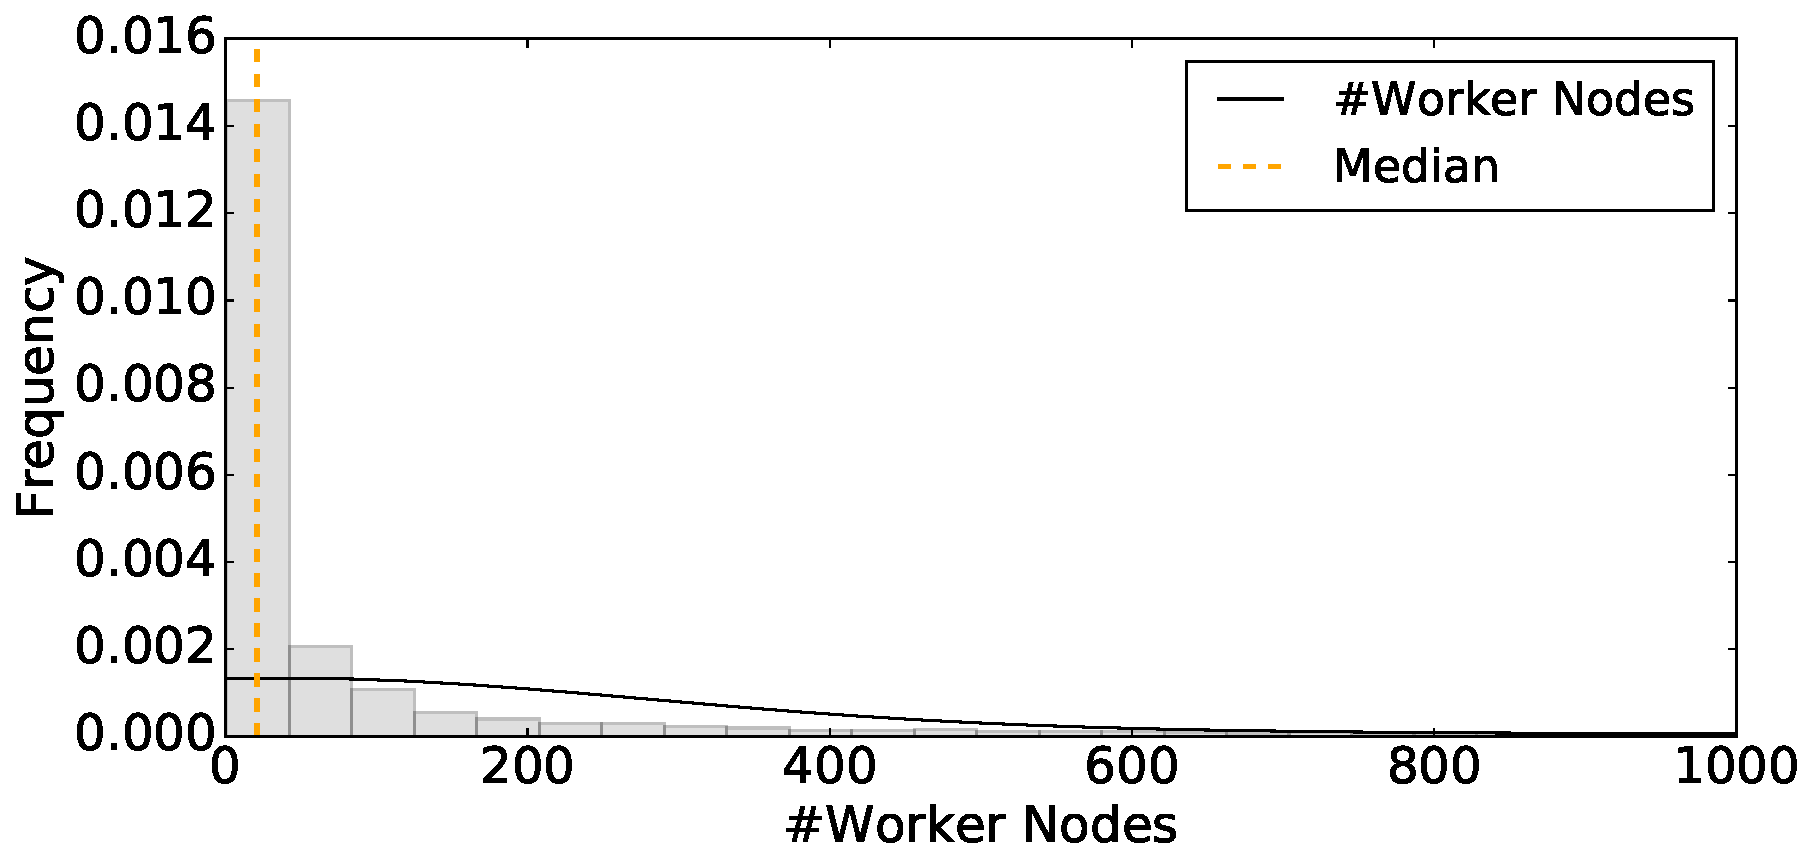
\includegraphics[clip,width=0.32\textwidth]{figures/titan_backfill_wnodes_distribution.pdf}
    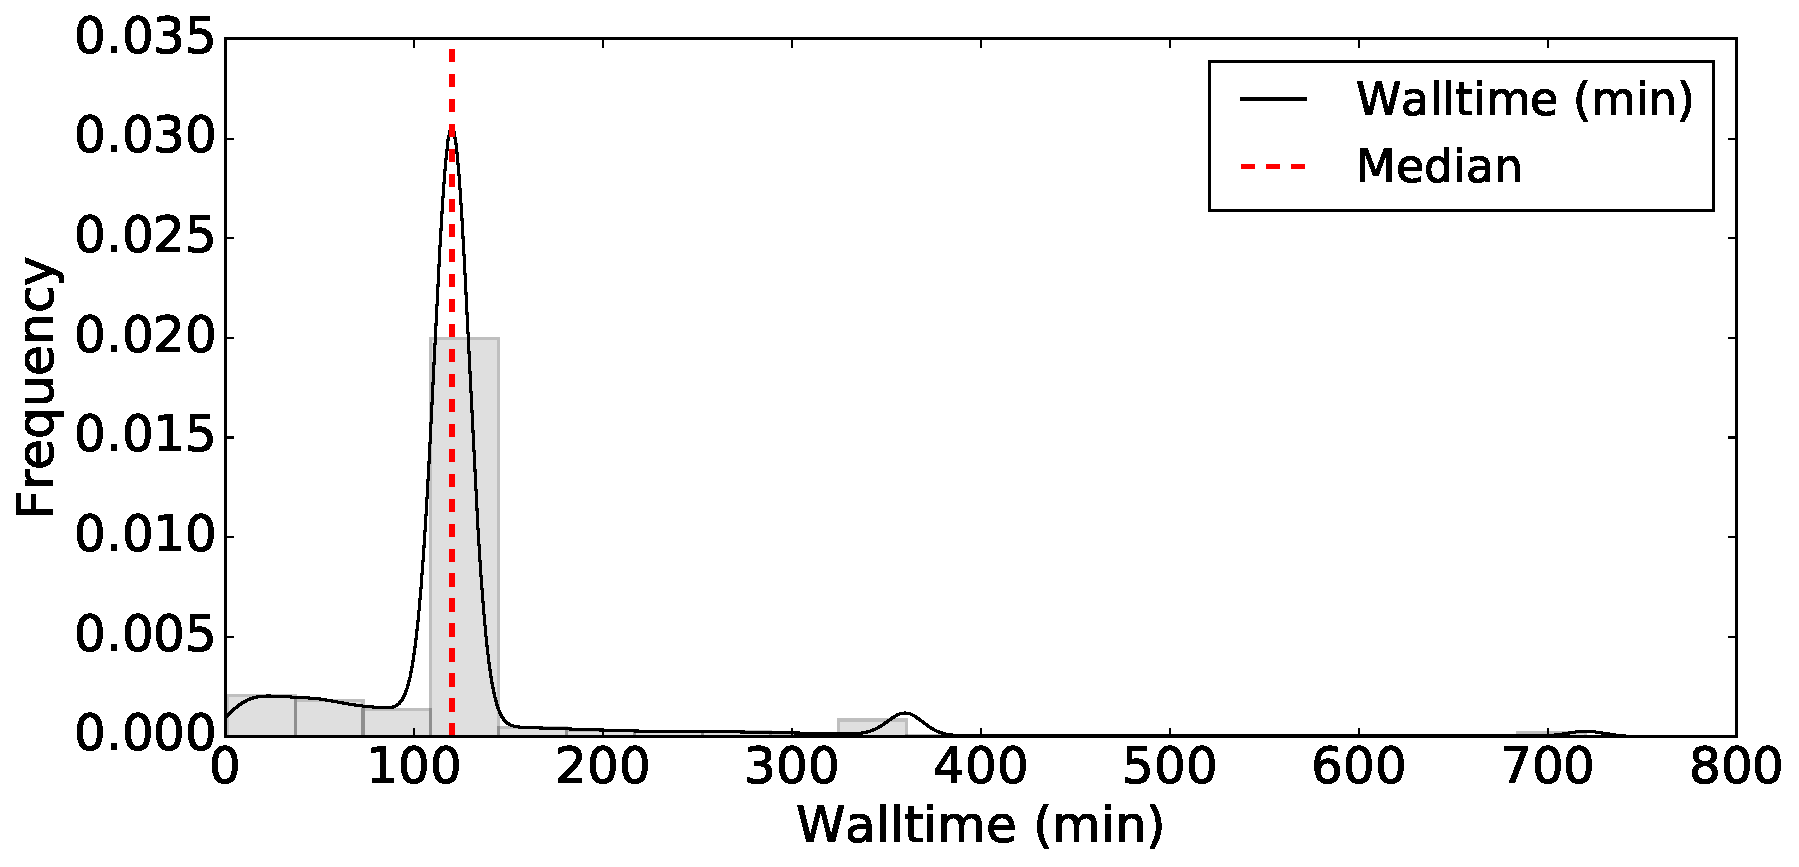
\includegraphics[clip,width=0.32\textwidth]{figures/titan_backfill_walltime_distribution.pdf}
    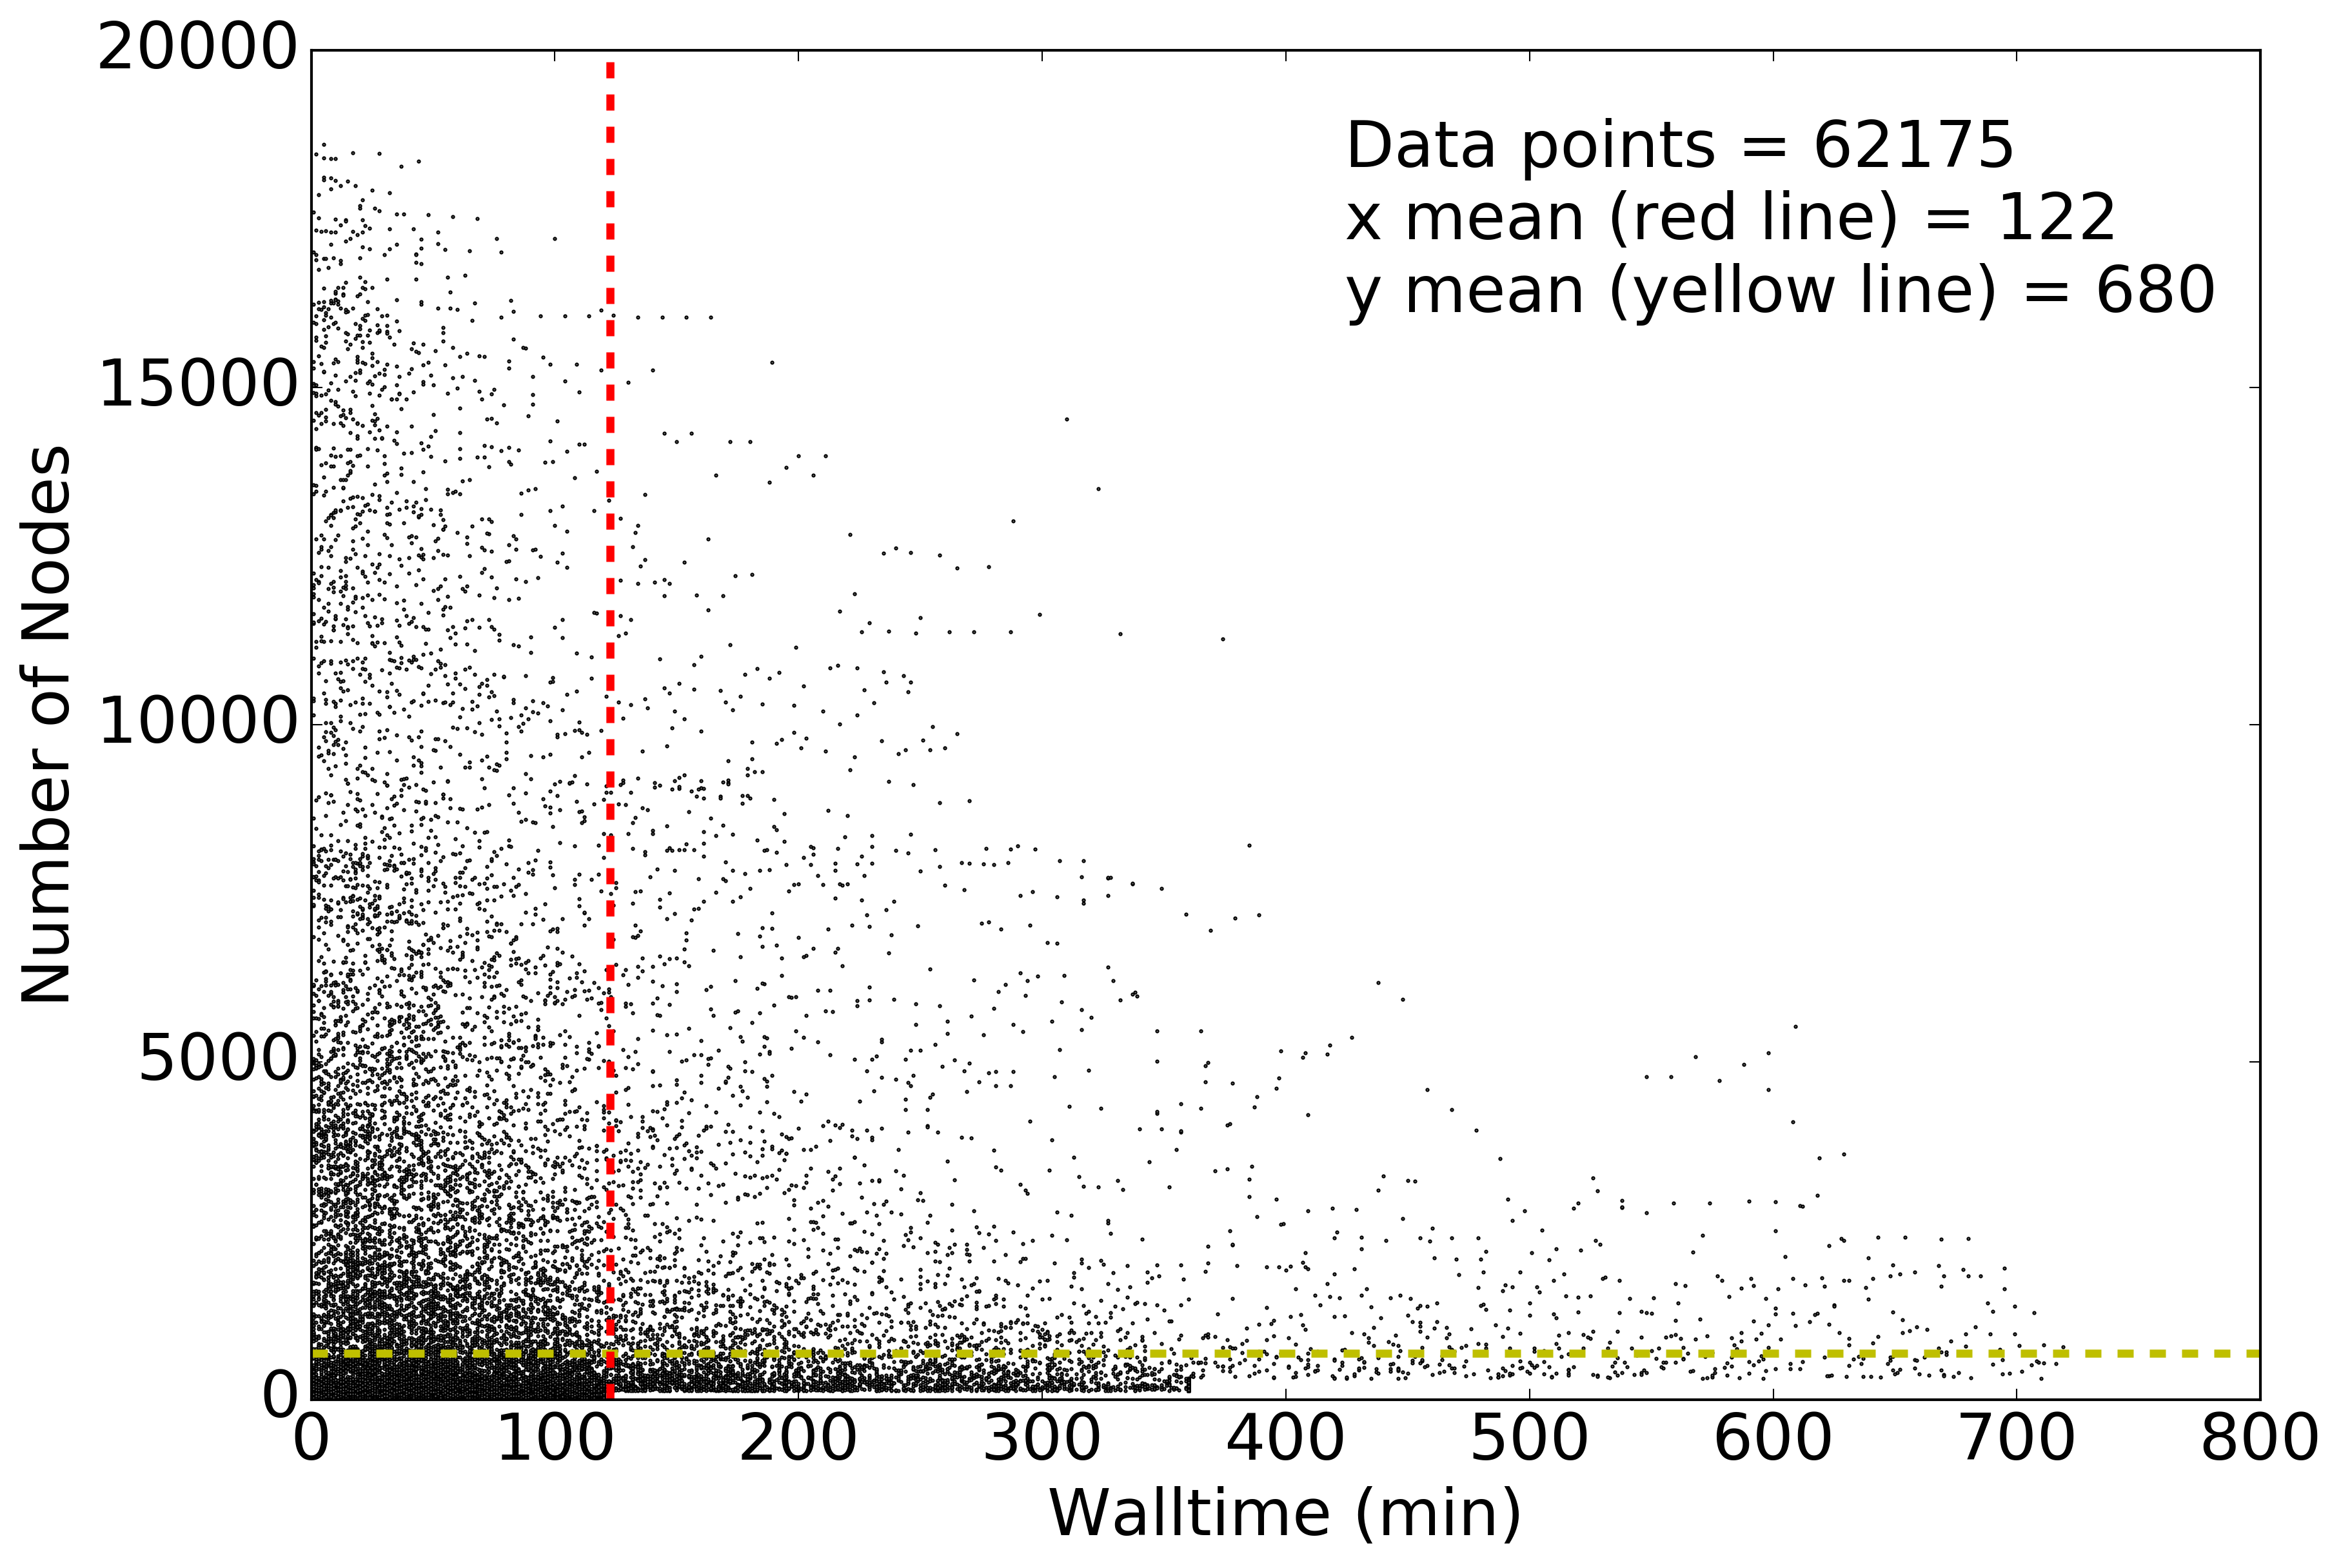
\includegraphics[clip,width=0.32\textwidth]{figures/titan_backfill_avail.png}
    %figures/avail_time_vs_nodes_Oct_28_Nov_3_2015.pdf}
    \caption{Backfill availability: distribution of number of work nodes (left);
    distribution of walltime in minutes (center); and a scatter plot of the two
    variables (right). 62175 measures: mean number of work nodes available 691;
    mean walltime available 126 minutes.}
\label{fig:backfill-distrib}
\end{figure*}

Usually, detector simulations performed on the Grid process 10 times the number
of events than those on Titan. This explains the difference between the
percentage of detector simulations and of events computed by those simulations
on Titan. PanDA Broker could fit the number of events to the walltime of the
backfill availability on the base of the distributions of
Fig.~\ref{fig:backfill-distrib}. That specific number of event could then be
pulled from the PanDA Event service~\cite{calafiura2015atlas} and given as input
to one or more simulations. Once packaged into the MPI script submitted to
titan's PBS batch system, these simulations would better fit backfill
availability, increasing the efficiency of PanDA Brokers.

The transition from a homogeneous to a heterogeneous number of events per
detector simulation has implications for the application layer. An even number
of events across simulations makes it easier to partition, track and package
events across simulations, especially when they are performed on both the Grid
and Titan. A homogeneous number of events also helps to keep the size and
duration of other stages of the MC workflow (\S\ref{ssec:panda-titan}) more
uniform. Further analysis is needed to evaluate the trade offs between increased
efficiency of resource utilization and the complexity that would be introduced
at the application layer.

Currently, each PanDA Broker creates, submits, and monitor a single MPI PBS
script at a time. This design is inherited from PanDA Pilot where a single
process is spawn at a time to execute the payload. As a consequence, the
utilization of a larger portion of Titan's total backfill availability depends
on the the number of concurrent PanDA Brokers instantiated on the DTNs: When all
the 20 PanDA Brokers have submitted a MPI PBS Job, further backfill availability
cannot be used.

In September 2016, increasing the number of concurrent PanDA Broker from 4 to 20
markedly improved efficiency (see Fig.~\ref{fig:backfill-utilization}) but
further research is undergoing to understand whether an even larger number
brokers would yield similar results. This research focuses on evaluating the the
overheads of input/output files staging, including its impact on DTNs, and on an
alternative design of PanDA Broker to enable the concurrent submission of
multiple MPI scripts~\cite{barreiro2016panda}.

% The number of concurrent detector simulation jobs that PanDA Broker can manage
% depends on the DTNs' resources. Each PanDA Broker can execute 1 MPI PBS job on
% up to 300 worker nodes for a total of 4,800 cores. Scaling above this
% threshold requires instantiating multiple PanDA Brokers on the same DTN and,
% once the DTN resources are saturated, on multiple DTNs.


% -----------------------------------------------------------------------------
\subsection{Characterizing the Detector Simulation on Titan}
\label{ssec:athenamp_titan}

% \begin{itemize}
%     \item problem with lustre addressed with ramdisk (done)
%     \item Competition for cache in AMD processors. (done)
%     \item Comparison hardware performance Titan/Grid (data acquired)
%     \item Summary overall figure of performance analogous to those produced
%     with NGE. Diagram as discussed in F2F meeting at Rutgers. (waiting)
% \end{itemize}

We use two main parameters to measure the performance of the detector simulation
jobs submitted to Titan: (i) the time taken to setup AthenaMP; and (ii) the
distribution of the time taken by the Geant4 toolkit to simulate a certain
number of events.

AthenaMP has an initialization and configuration stage. At initialization time,
AthenaMP is assembled from a large number of shared libraries, depending on the
type of payload that will have to be computed. Once initialized, every algorithm
and service of AthenaMP is configured by a set of Python scripts. Both these
operations result in a large number of read operations on the filesystem shared
between the worker nodes and the DTNs, including the operations required to
access of small python scripts.

% AthenaMP is a multipurpose framework that needs to be configured depending on
% the type of payalod that needs to be executed. For Geant4, this configuration
% process links up to 200 libraries, all requiring filesystem read and write
% operations.

% The execution of Geant4 is mostly compute-intensive requiring to write around
% XXKB per 100 events on disk and no more than 2GB of memory.

% -----------------------------------------------------------------------------
% \subsection{PanDA Shared Library I/O Performance Impact at OLCF}

% Athena, the ATLAS framework has a configuration and initialization stage. At
% this stage, the running job is assembled on the fly from a large number of
% shared libraries. Also, at this stage, every algorithm and service is being
% configured, at run time, by a corresponding set of Python scripts, which
% results in a large number of read operations accesses to small python
% scripts, with many includes and imports Python calls.

% \mtnote{TODO: specify that this is work in progress (see Sergey's comment) and
% see how to move it to the data performance subsection}

Initially, all the shared libraries of AthenaMP and the python scripts for the
configuration stage were stored on the Spider 2 Lustre file system. However, the
I/O patterns of the initialization and configuration stages degraded the
performance of the filesystem.
% (Figure~\ref{}\mtnote{We may want to aggregate some of the diagrams about
% lustre's experiments here}).  Since Spider 2 is a center-wide file system,
% this resulted in  performance degradation for all OLCF resources and users.
% \mtnote{I am afraid the details about the trace are too specific given the
% space constraints of a SC  submission. Please feel free to uncomment it if
% you disagree.}
%
% As can be seen in Listing~\ref{mdstrace} the metadata I/O activity for ATLAS
% exhibits a spike corresponding to the beginning of the runs before tapering
% off.
%
% \begin{minipage}{\linewidth}
% \begin{lstlisting}[language=bash,frame=single,basicstyle=\ttfamily\tiny,caption=ATLAS metadata trace,label=mdstrace]
% XK7 Application 9205593
%       39012 RPCs from 300 of 300 nodes
%         ~69291.96 per sec
%           37851 LDLM_ENQUEUE RPCs    ~67229.83 per sec
%                 pmin 13us pavg 42us pmax 4983us
%           611 LDLM_CANCEL RPCs    ~1085.24 per sec
%                 pmin 10us pavg 16us pmax 32us
%           277 MDS_CLOSE RPCs    ~492.00 per sec
%                 pmin 15us pavg 20us pmax 38us
%           154 MDS_READPAGE RPCs    ~273.53 per sec
%                 pmin 170us pavg 292us pmax 671us
%           86 MDS_GETXATTR RPCs    ~152.75 per sec
%                 pmin 15us pavg 21us pmax 65us
%           30 MDS_GETATTR RPCs    ~53.29 per sec
%                 pmin 16us pavg 20us pmax 27us
%           3 MDS_REINT RPCs    ~5.33 per sec
%                 pmin 103us pavg 136us pmax 196us
%           Overall times
%                 pmin 10us pavg 42us pmax 4983us
%
% XK7 Application 9205355
%       8698 RPCs from 62 of 62 nodes
%         ~15449.13 per sec
%           8445 LDLM_ENQUEUE RPCs    ~14999.76 per sec
%                 pmin 16us pavg 41us pmax 780us
%           92 MDS_CLOSE RPCs    ~163.41 per sec
%                 pmin 15us pavg 23us pmax 52us
%           55 MDS_READPAGE RPCs    ~97.69 per sec
%                 pmin 189us pavg 291us pmax 534us
%           52 LDLM_CANCEL RPCs    ~92.36 per sec
%                 pmin 12us pavg 16us pmax 25us
%           41 MDS_GETXATTR RPCs    ~72.82 per sec
%                 pmin 16us pavg 20us pmax 27us
%           13 MDS_GETATTR RPCs    ~23.09 per sec
%                 pmin 16us pavg 21us pmax 38us
%           Overall times
%                 pmin 12us pavg 42us pmax 780us
%
% \end{lstlisting}
% \end{minipage}
%
% As this problem was identified, the OLCF staff has enabled read-only access to
% certain NFS-exported directories from Titan compute nodes. This in turn
% allowed the OLCF staff to install a software package from a Titan login node
% and have it available read-only on a Titan compute node.
%
% After careful characterization of the impact of ATLAS jobs on Lustre, the
% performance degradation
This was addressed by moving the AthenaMP distribution to a read-only NFS
directory, shared among DTNs and worker nodes. NFS eliminated the problem of
metadata contention, improving metadata read performance from $\approx$6,300
seconds on Lustre to $\approx$1,500 seconds on NFS.

% Figure~\ref{fig:atlas-perf-improvement} shows the overall ATLAS performance
% improvement on Titan. The circled region illustrates the switch from Lustre to
% NFS-exported directory for hosting the ATLAS release.

%\begin{figure}[!htb]
%    \centering
%    \begin{tabular}{cc}
%        {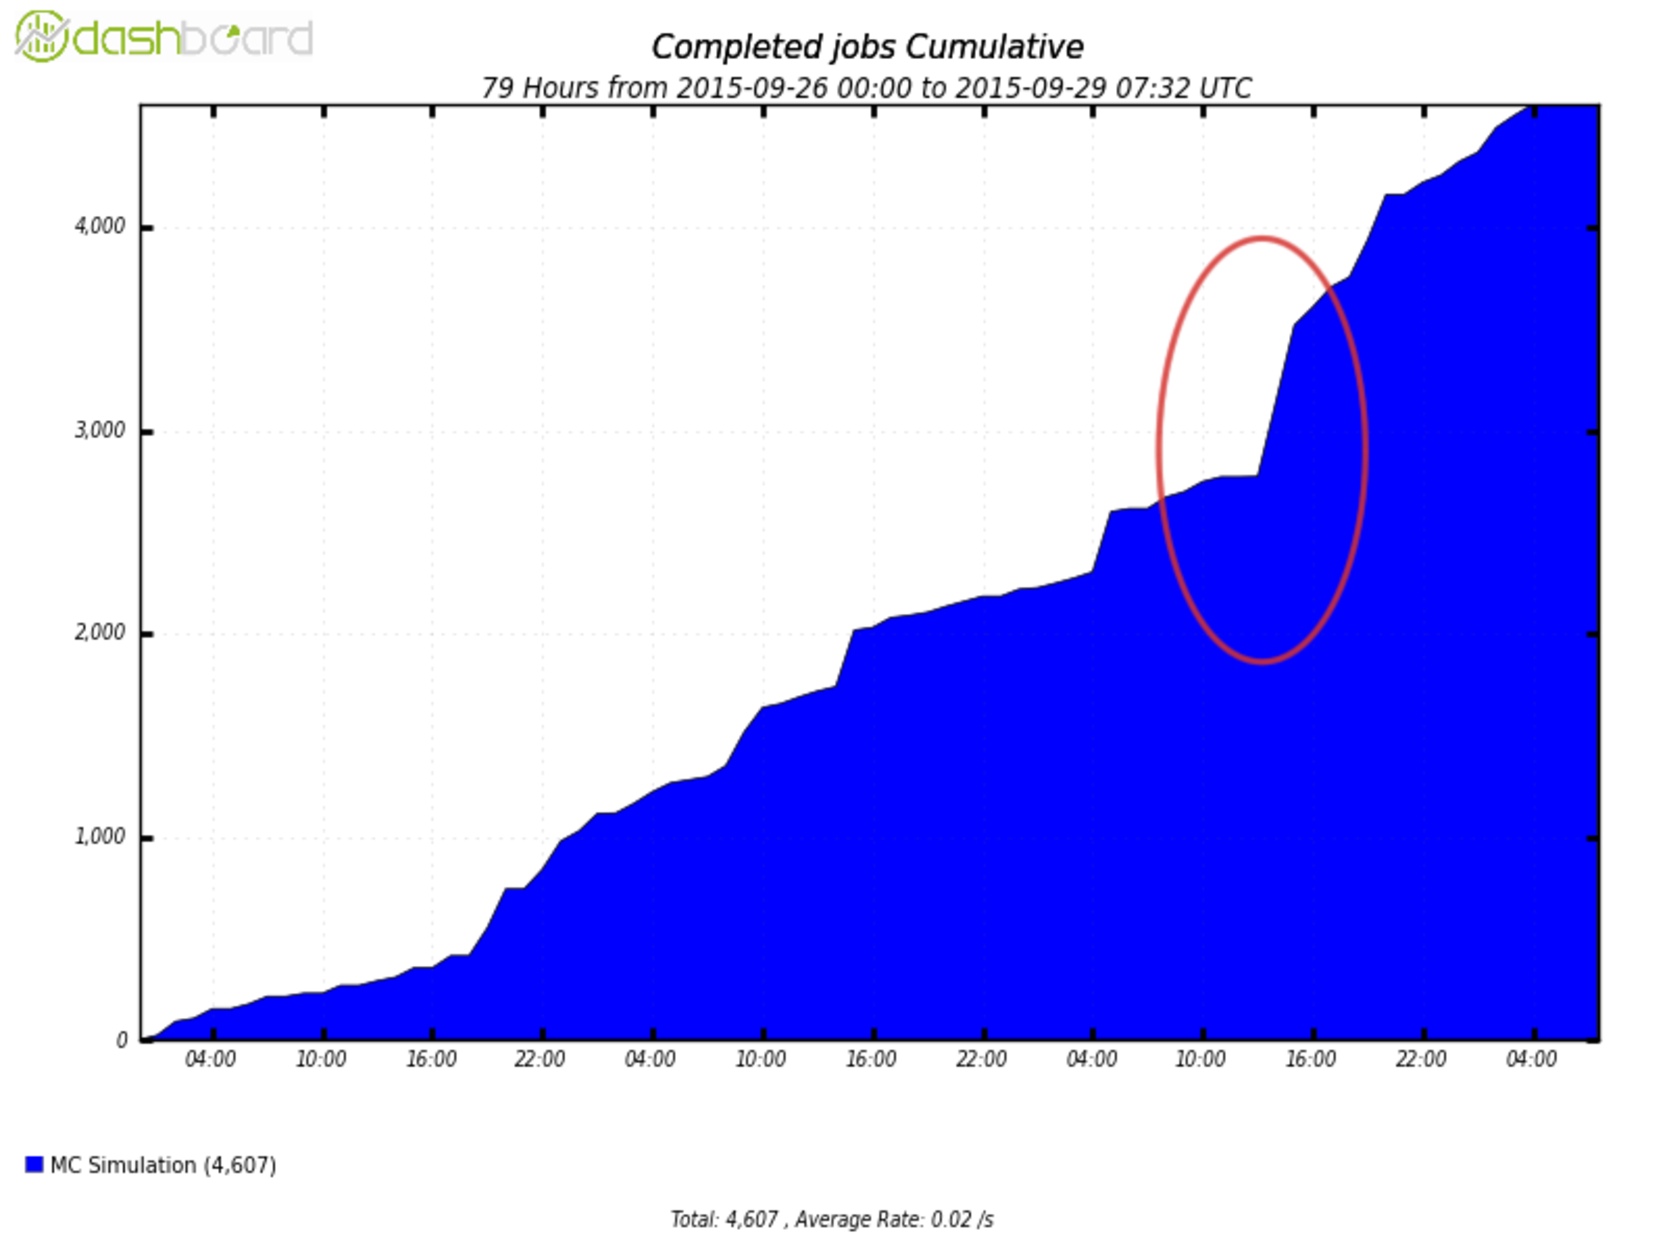
\includegraphics[width=0.48\textwidth]{figures/panda-completed-jobs-sw-move.pdf}}\\
%    \end{tabular}
%    \caption{ATLAS performance improvement on Titan. The circled region shows the switch from Lustre to NFS-exported directory for hosting the ATLAS release.}
%\label{fig:atlas-perf-improvement}
%\end{figure}

Once set up, AthenaMP is used to execute 16 concurrent Geant4 simulators on each
of Titan's worker node. Geant4 requires to read events descriptions from a
filesystem and simulate them as they would happen within the ATLAS detector. We
characterized both the compute performance of the simulation and the impact of
acquiring event descriptions on the filesystem.

The AMD Opteron 6274 CPU used on Titan has 16 cores, divided into 8 compute
units. Each compute units has 1 floating point (FP) scheduler shared between 2
cores. When using 16 cores for FP-intensive calculations, each pair of cores
competes for a single FP scheduler. This creates the overhead shown in
Figure~\ref{fig:comparison-8-16cores}: the mean runtime per event for 8
concurrent simulations computing 50 events is 10.8 minutes, while for 16
simulations is 14.25 minutes (consistent with the measured distribution of the
duration of event simulation). Despite an inefficiency of almost 30\%, Titan's
allocation policy based on number of worker nodes used instead of number of
cores does not justify the use of 1/2 of the cores available.

\begin{figure}[htp]
    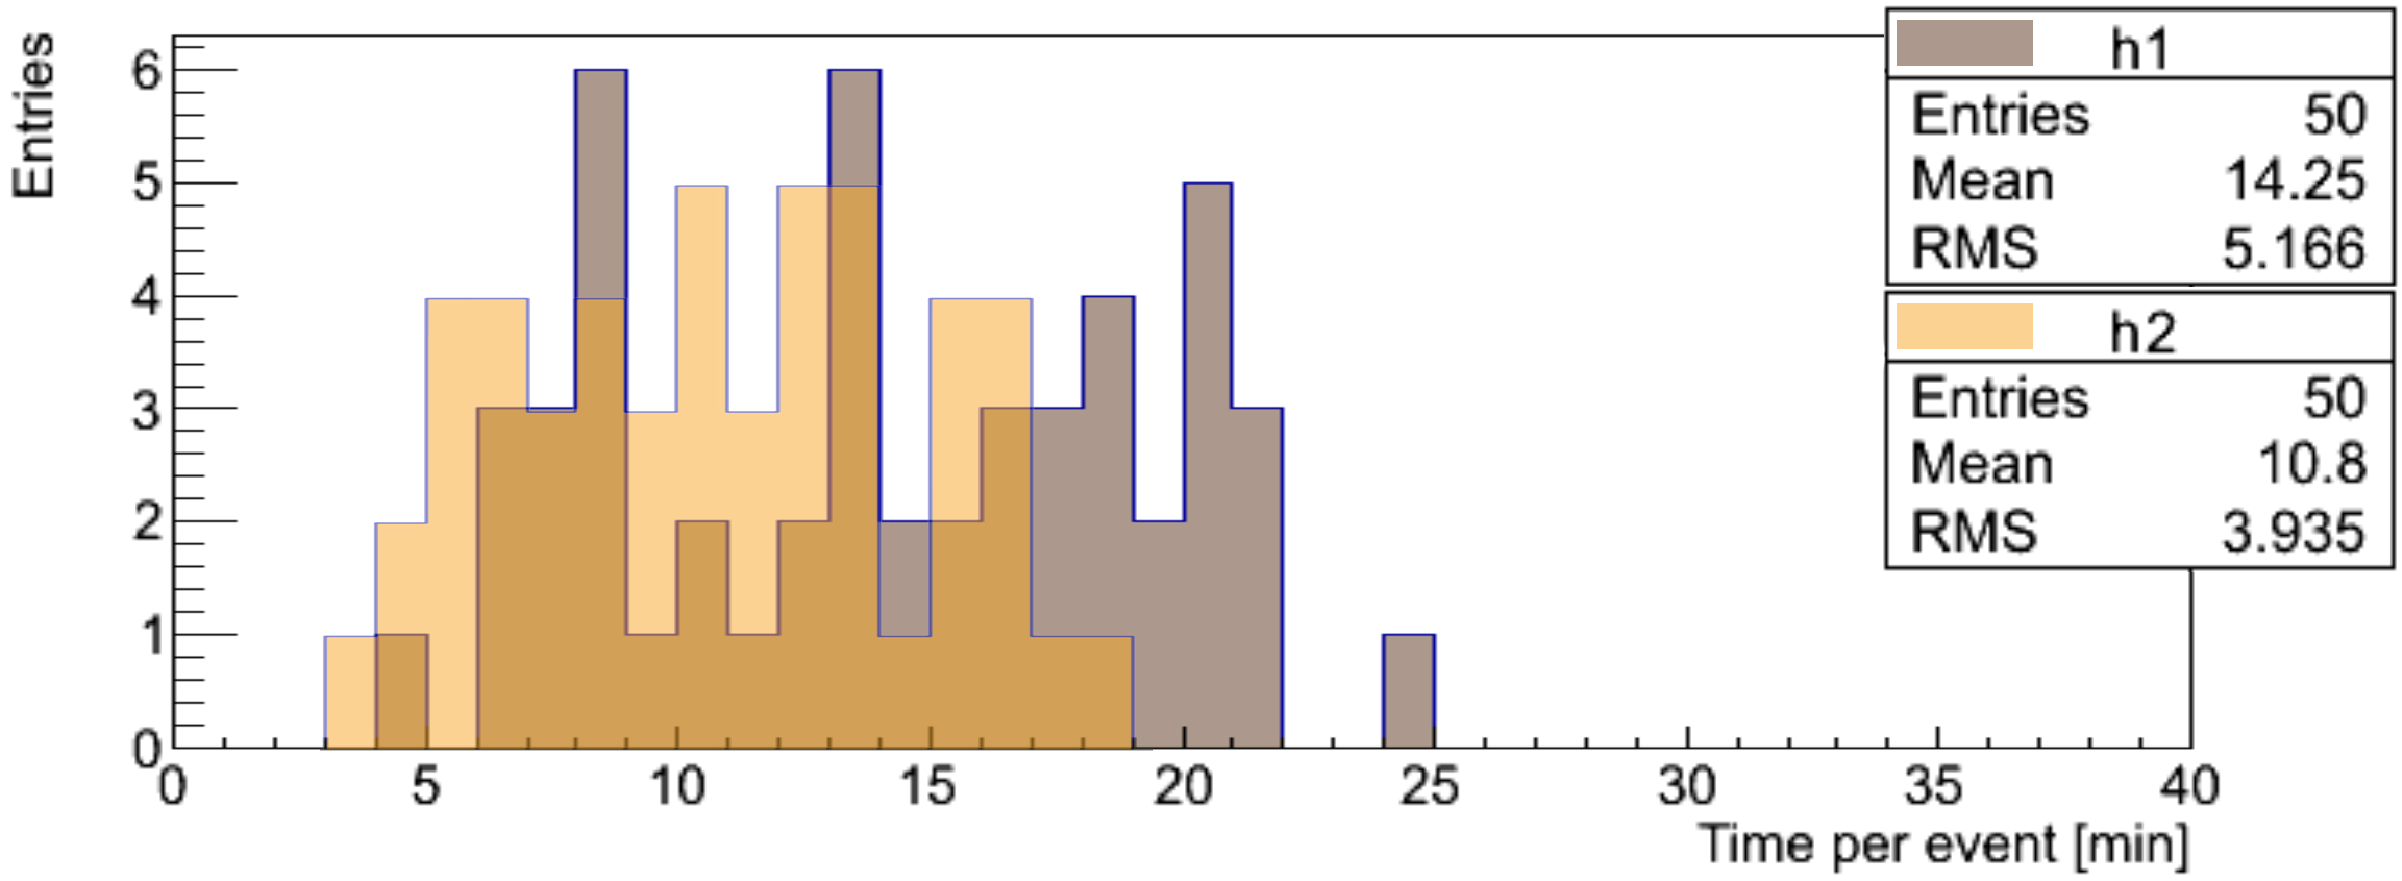
\includegraphics[clip,width=\columnwidth]{figures/tx8_tx16_comparison_vsquashed.pdf}
    \caption{Comparison between distributions of the time taken by a Geant4
    detector simulation to simulate one event when placing 2 simulations (h1) or
    1 simulation (h2) per CPU. 2 simulation use 16 cores per node, 1 simulation
    8, 1 per compute unit. 50 Events; 1 Titan worker nodes; 16 work threads per
    node; 100 events per node.}
\label{fig:comparison-8-16cores}
\end{figure}

The performance analysis of Titan's AMD CPUs for detector simulations helps also
to compare Titan and Grid site performances. Usually, Grid sites exposes
resources with heterogeneous CPU architectures and a maximum of 8 (virtual)
cores per worker node, while Titan's offer an homogeneous 16 cores architecture.
We used the rate of events processes per minute as a measure of the efficiency
of executing the same detector simulation on both Titan or Grid sites.
% Figure~\ref{fig:comparison-titan-grid} compares the efficiencies of Titan to
% the BNL and SIGNET Grid sites, normalized for 8 cores. Effective performance
% per-core at Titan is $\approx$0.57 event per minute, roughly 1/2 of BNL and
% 1/3 of SIGNET performances.
Comparisons of the efficiencies of Titan to  the BNL and SIGNET Grid sites,
normalized for 8 cores, show that the effective performance per-core at Titan is
$\approx$0.57 event per minute, roughly 1/2 of BNL and  1/3 of SIGNET
performances.

% \begin{figure}[htp]
%     \includegraphics[clip,width=\columnwidth]{figures/titan_grid_event_rate.pdf}
%     \caption{Comparison of the event rate for finished jobs at Titan (h1), BNL
%     (h2) and GRIDNET (h3). Titan histogram shows 1/2 of the measured values to
%     account for the core difference between Titan (16) and the Grid sites (8).
%     Performance per core: BNL 1.126; SIGNET 0.885; Titan 0.577.\mtnote{TO BE DELETED.}}
% \label{fig:comparison-titan-grid}
% \end{figure}

The differences in performance between Titan and the BNL and SIGNET Grid sites
are due to the FP scheduler competition and the availability of newer
processors. The CPUs at the Grid sites have one FP scheduler per core and are on
average newer than the CPU of Titan. The heterogeneity of the Grid sites' CPUs
explain the higher performance variance compared to the performance consistency
measured on Titan.

% \mtnote{Figure summarizing job performance on Titan analogous to those
% produced with NGE, as discussed in F2F meeting at Rutgers?}
%
% ----------------------------------------------------------------------------
% \subsection{Reliability of PanDA Broker and Detector Simulations on Titan}
% \label{ssec:reliability}
%
% Figure~\ref{fig:failures-titan} shows a breakdown of the type of failures
% recorded by the PanDA Brokers between January 2016 and February 2017. The
% initial preponderance of unknown failures was progressively addressed by a
% more accurate failure model, specifically tailored to the PanDA Broker and
% Titan. Figure~\ref{fig:failures-titan} also shows the progressive improvement
% of the broker's reliability: In Februrary 2017, errors related to input files
% and initialization were almost eliminated and execution errors were comparable
% to those recorded in January 2017 even if almost twice as many simulations
% were performed (Figure~\ref{fig:backfill-utilization}). The increased amount
% of unknown failure in February indicates that furter work is needed to improve
% the PanDA Broker failure model.
%
% \begin{figure}[htp]
%     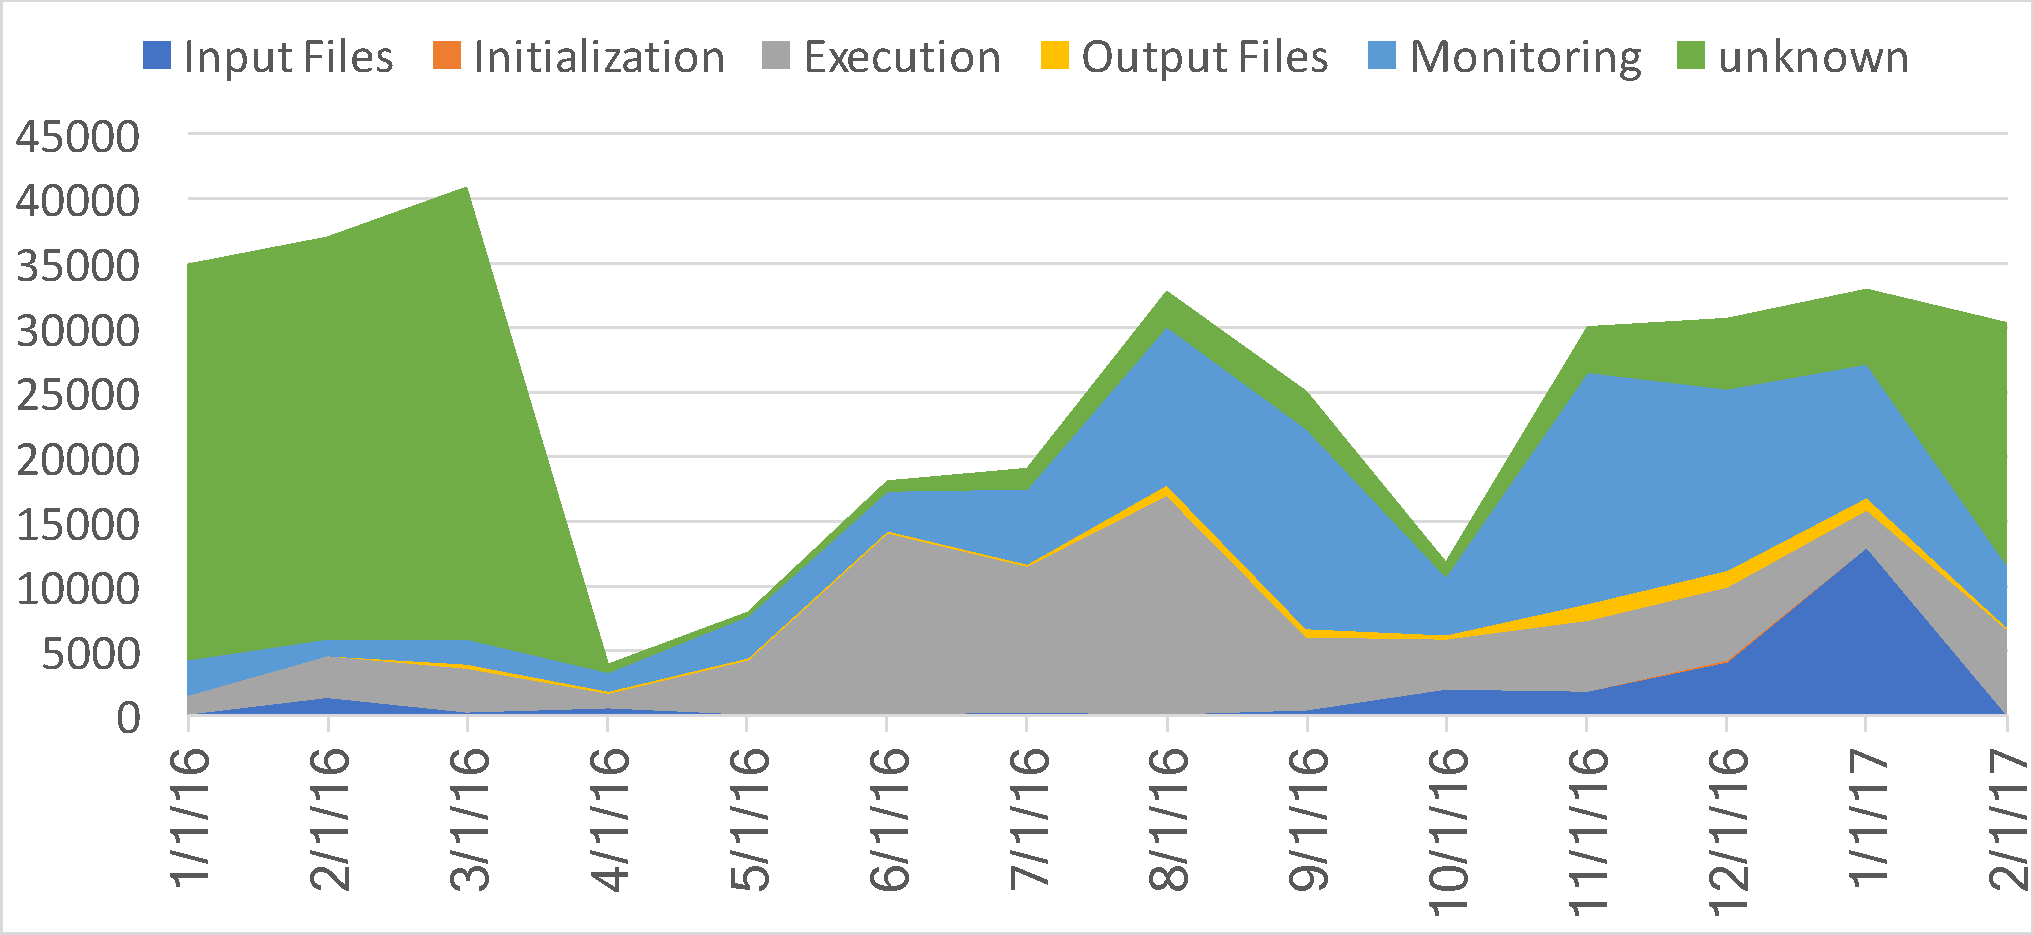
\includegraphics[clip,width=\columnwidth]{figures/failures_titan.pdf}
    % \caption{PanDA Broker failures during the experiment time window. Failures
    % were recorded with 52 exit codes, here aggregated into 6 categories. The
    % number of failures should be compared to the number of simulations
    % executed in each month as plotted in
    % Figure~\ref{fig:backfill-utilization}. Improvements in the failure model
    % of PanDA Broker shows a decrease in unknown failure and a the progressive
    % addressing of other categories of failure.}
% \label{fig:failures-titan}
% \end{figure}
%
% -----------------------------------------------------------------------------
% \subsection{Characterizing PanDA I/O}
%
% To better understand the I/O impact of ATLAS PanDA project on Titan
% supercomputing environment

We studied the impact of acquiring event descriptions on Lustre by analyzing
1,175 jobs ran on the week of 10/25/2016, for a total of 174 hours.
Table~\ref{panda-olcf-stats} shows the overall statistical breakdown of the
observed file I/O.
% Figures~\ref{fig:atlas-titan-io-read} and~\ref{fig:atlas-titan-io-written}
% show the file read and write I/O histograms for these 1,175 jobs,
% respectively. Figures~\ref{fig:atlas-titan-file-open}
% and~\ref{fig:atlas-titan-file-close} show the file $open()$ and $close()$
% metadata load histograms of the same  1,175 ATLAS jobs, respectively.
%
% As can be seen from Table~\ref{panda-olcf-stats},
%
ATLAS used between 1 and 300 worker nodes, and 35 on average. 75\% of the jobs
run by ATLAS consumed less than 25 nodes and 92\% less than 100. During the 174
hours of data collection, 6.75 ATLAS jobs were executed on average per hour,
each job running for an average of 1.74 hours.
% ATLAS jobs issues a large number of file read operations, as can be seen in
% Table~\ref{panda-olcf-stats}.
Every job read less than 250 GB and wrote less than 75 GB of data and, on
average, each job read 20 GB and wrote 6 GB of data.

\begin{table*}[t]
\centering
\begin{tabular}{lllllllll}
 & Num. Nodes & Duration (s) & Read (GB) & Written (GB) & GB Read/nodes & GB Written/nodes & $open()$ & $close()$ \\
Min & 1 & 1,932 & 0.01 & 0.03 & 0.00037 & 0.02485 & 1,368 & 349 \\
Max & 300 & 7,452 & 241.06 & 71.71 & 0.81670 & 0.23903 & 1,260,185 & 294,908 \\
Average & 35.66 & 6,280.82 & 20.36 & 6.87 & 0.38354 & 0.16794 & 146,459.37 & 34,155.74 \\
Std. Dev. & 55.33 & 520.99 & 43.90 & 12.33 & 0.19379 & 0.03376 & 231,346.55 & 53,799.08
\end{tabular}
\caption{The Statistical breakdown of the I/O impact of 1,175 jobs ATLAS executed at OLCF for the week of 10/25/16}
\label{panda-olcf-stats}
\end{table*}

% \begin{figure}[!htb]
%     \centering
%     \begin{tabular}{cc}
%         {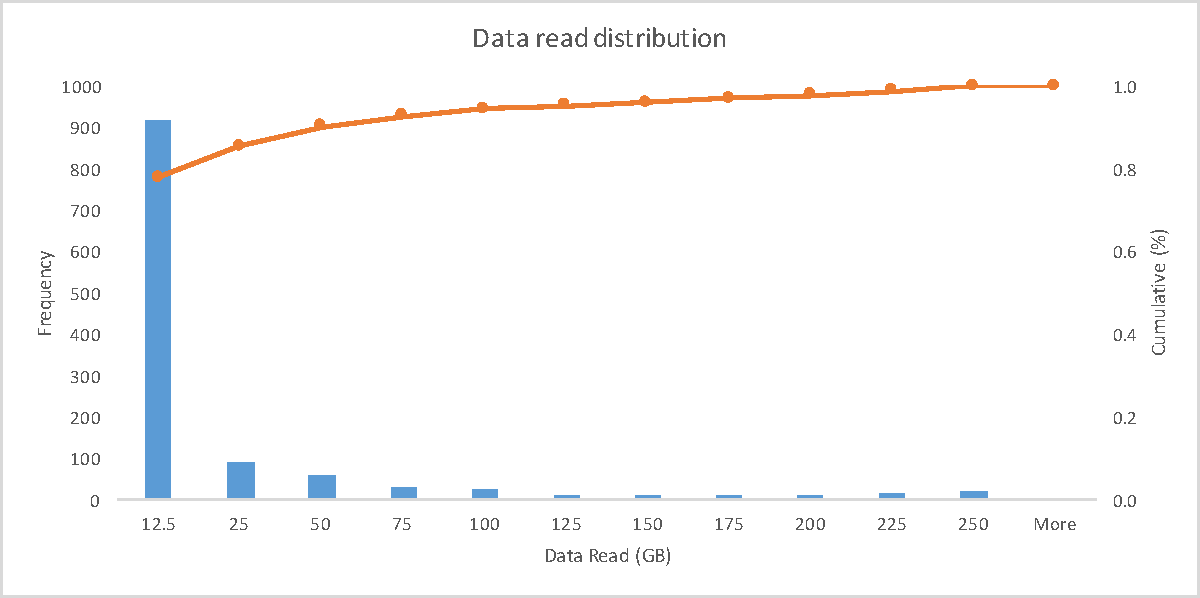
\includegraphics[width=0.48\textwidth]{figures/panda_data_read_finer_hist.pdf}}\\
%     \end{tabular}
%     \caption{ATLAS file read operation histogram on Titan for week of 10/25/16.}
% \label{fig:atlas-titan-io-read}
% \end{figure}
%
% \begin{figure}[!htb]
%     \centering
%     \begin{tabular}{cc}
%         {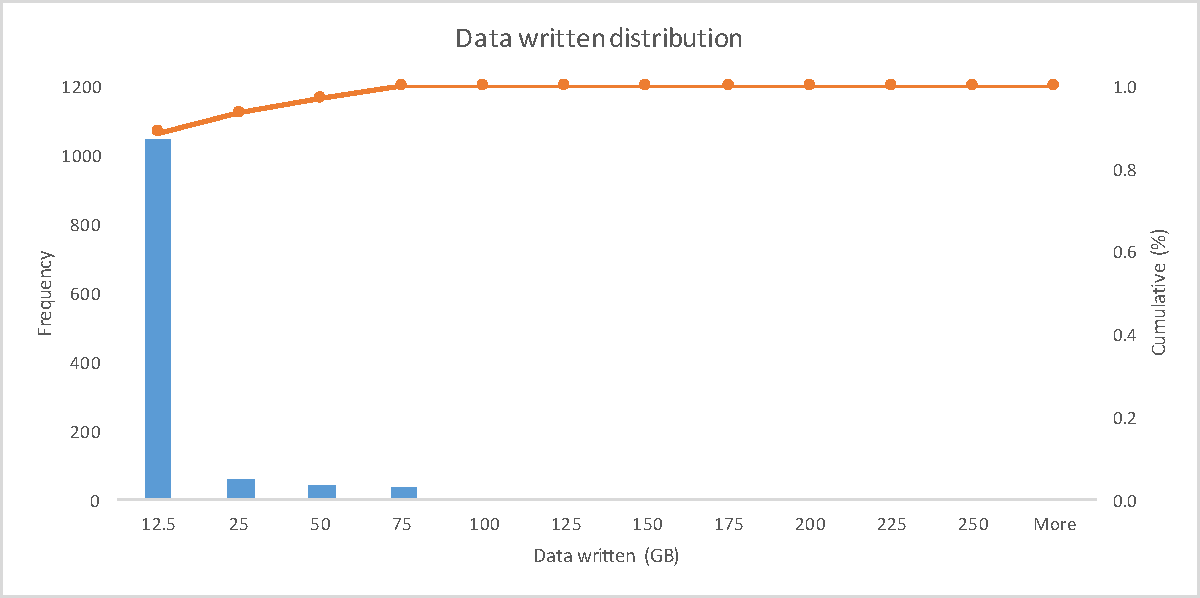
\includegraphics[width=0.48\textwidth]{figures/panda_data_written_finer_hist.pdf}}\\
%     \end{tabular}
%     \caption{ATLAS file write I/O histogram on Titan for week of 10/25/16.}
% \label{fig:atlas-titan-io-written}
% \end{figure}

% The I/O of the ATLAS jobs show an interesting pattern.
% Table~\ref{panda-olcf-stats} indicates that the amount of data read per ATLAS
% worker node is less than 400 MB on average, while the amount of data written
% per node is less than 170 MB on average. This correlates with our finding
% that ATLAS PanDA jobs are read heavy. However,

ATLAS jobs are read heavy: On average, the amount of data read per worker node
is less than 400 MB, while the amount of data written is less than 170 MB.
% as can be seen in Table~\ref{panda-olcf-stats} and figures
% {fig:atlas-titan-io-read} and {fig:atlas-titan-io-written},
Distributions of read and written data are different: The read operation
distribution per job shows a long tail, ranging from 12.5 GB to 250 GB, while
the written amount of data has a very narrow distribution.

% \begin{figure}[!htb]
%     \centering
%     \begin{tabular}{cc}
%         {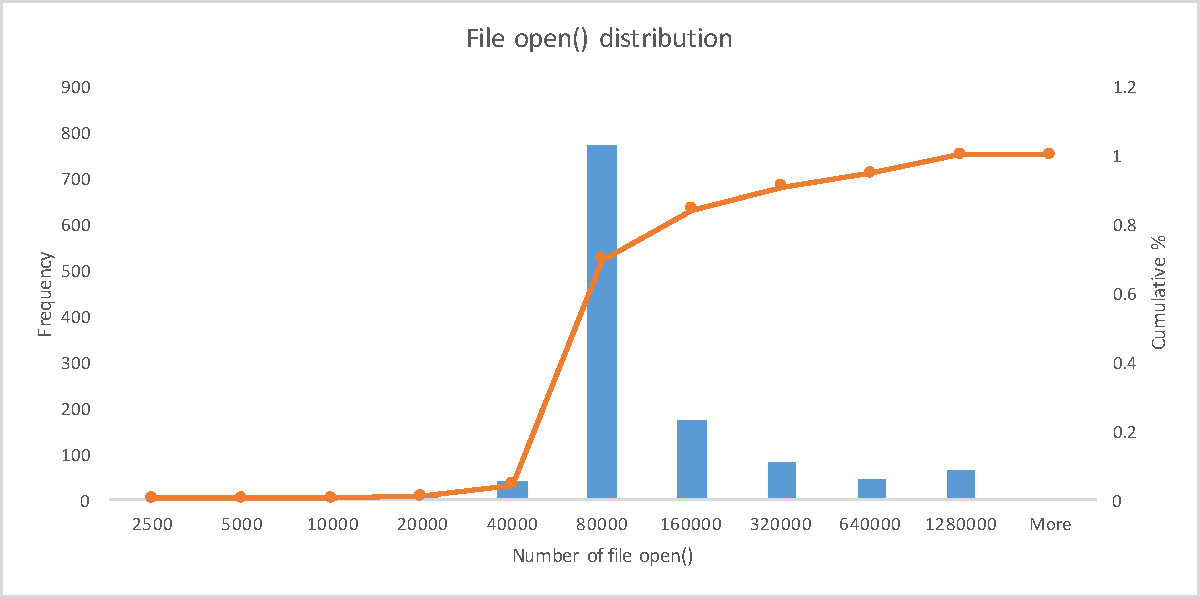
\includegraphics[width=0.48\textwidth]{figures/panda_file_open_hist.pdf}}\\
%     \end{tabular}
%     \caption{ATLAS file $open()$ histogram on Titan for week of 10/25/16.}
% \label{fig:atlas-titan-file-open}
% \end{figure}
%
% \begin{figure}[!htb]
%     \centering
%     \begin{tabular}{cc}
%         {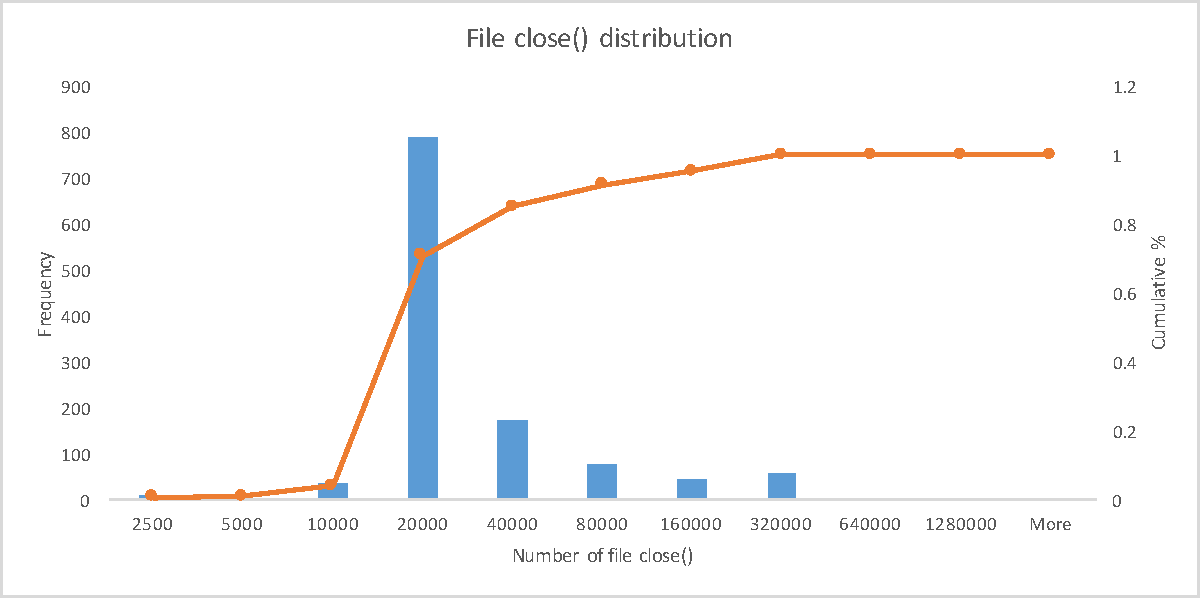
\includegraphics[width=0.48\textwidth]{figures/panda_file_close_hist.pdf}}\\
%     \end{tabular}
%     \caption{ATLAS file $close()$ histogram on Titan for week of 10/25/16.}
% \label{fig:atlas-titan-file-close}
% \end{figure}

The metadata I/O breakdown shows that ATLAS jobs yield 23 file $open()$
operations per second (not including file $stat()$ operations) and 5 file $close()$ operations per second, with similar distributions.
% As can be seen from figures~\ref{fig:atlas-titan-file-open}
% and~\ref{fig:atlas-titan-file-close}, they .
On average, the maximum number of file $open()$ operations per job is
$\approx$170/s and the maximum number of file $close()$ operations is
$\approx$39/s.
% on average per second per job.
For the 1,175 ATLAS jobs observed, the total number of file $open()$ operations
is 172,089,760 and the total number of file $close()$ operations is 40,132,992.
The difference between these two values is still under investigation: One
possible explanation is that ATLAS jobs don't call a file $close()$ operation
per every file $open()$ issued.

% based on our experiments with ATLAS jobs, it can be safely concluded
% that the file and metadata I/O load of ATLAS PanDA project on the OLCF Titan
% supercomputing environment and the Spider 2 file system is not detrimental to
% the center operations. At the current scale of the project, the overall impact
% of ATLAS operations on Titan is minimal.

Overall, the average time taken to read events from input files stored on Lustre is 1,320, comparable to the time taken to read the file required by assembling AthenaMP from NFS. Preliminary investigation shows that this time could be reduced to 40 seconds by loading the event descriptions into the RAM disk available on each worker node. Events descriptions could be transferred from Lustre to the RAM disk while configuring and initializing AthenaMP, almost halving the time currently required by initiating a Genat4 simulation.

The current design and architecture of the PanDA Broker is proving to be as
reliable as PanDA Pilot when used on the WLCG. Between Jan 2016 and Feb 2017,
the overall failure rate of all the ATLAS detector simulation jobs was 14\%,
while the failure rate of jobs submitted to Titan was a comparable 13.6\%. PanDA
Brokers were responsible for around the 19\% of the failures, compared to the
29\% of failures produced by the JobDispatcher module of the PanDA Server, and
the 13\% failures produced by the Geant4 toolkit. The current failure rate of
the PanDA Brokers confirms the benefits of reusing most of the code base of the
PanDA Pilot for implementing the PanDA Broker. It also shows that adopting
third-party libraries like RADICAL-SAGA did not have a measurable adverse effect
on reliability.


%\section{Putting it all together: Experience of PanDA on TITAN} % (fold)
%\label{sec:panda_titan}
%
%\begin{enumerate}
%  \item Metadata performance issue, and how it’s resolved
%  \item File I/O performance and impact
%  \item ?
%\end{enumerate}


% ----------------------------------------------------------------------------
% VII - THE NEXT GENERATION EXECUTOR
% ----------------------------------------------------------------------------
% \section{PANDA: Future/RoadMap}
\section{PANDA\@: The Next Generation Executor}
\label{sec:panda_roadmap}

\begin{enumerate}
    \item Discussion of the limitations of the current state of the art
    \item Rationale and design (why)
    \item Architecture (how)
    \item Integration
    \item Characterization (experiments)
\end{enumerate}

\subsection{Experiments}
\label{sec:ngeExp}

We designed experiments to characterize the performance of the NGE on Titan,
with an emphasis on understanding its overhead and thus the cost of introducing
new functionalities.  We perform three groups of experiments in which we
investigate the weak scalability, weak scalability with multiple generation, and
strong scalability of the NGE.

Each experiment entails executing multiple instances of AthenaMP 
to simulate a pre-determined number of events. All the experiments have been
performed by  configuring AthenaMP to use all the 16 cores  of Titan's worker
nodes.

We  measured the execution time of the pilots and of AthenaMP 
within them, collecting timestamps at  all stages of the execution. Experiments
were performed  by  submitting NGE's pilots  to Titan's batch queue.  The
turnaround time of an individual run is determined by queue waiting times. Since
we are interested only in the performances of the NGE, we removed queue time
from our statistics.

\subsubsection{Weak scalability}

In this experiment  we run as many AthenaMP instances (hereafter referred to as
tasks)  as the number of nodes controlled by the pilot. Each AthenaMP simulates
100 events, requiring $\sim 4200$ seconds on average.

Tasks do not  wait within the NGE Agent's queue since  one node  is available to
each AthenaMP instance.  Overheads in task execution are consequence primarily
of the three other factors: (i) the  initial bootstrapping of the pilot on the
nodes; (ii) the UnitManager's dispatching of  units (tasks) to the agent; and
(iii) time for the agent to bootstrap all the tasks on the nodes.

We tested  pilots  with 250, 500, 1000 and 2000 worker nodes and 2 hours
walltime. The time duration is determined by the Titan's walltime policy.
Fig.~\ref{fig:weakScal1a} depicts the average pilot duration, the average
execution time of AthenaMP, and the NGE pilot overhead as function of the pilot
size.

\begin{figure}[!htb]
        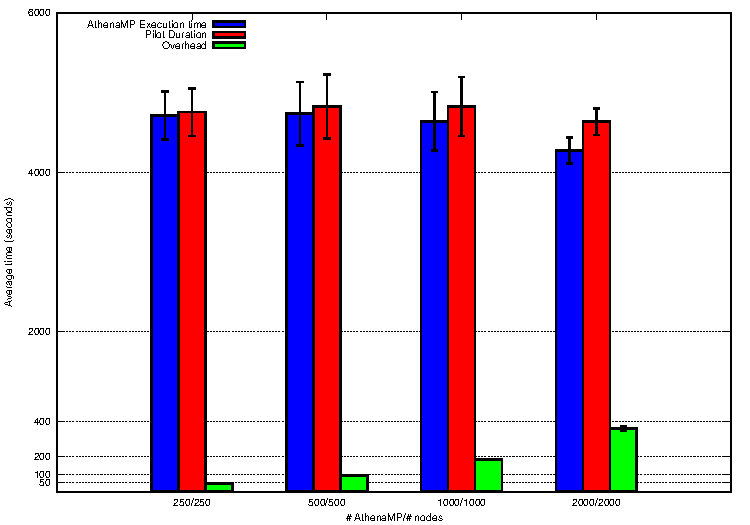
\includegraphics[height=4.5cm,width=\columnwidth]{./figures/NGE/weak1.pdf}
    \caption{Weak scalability: average pilot duration, average duration of one AthenaMP execution, and pilot's overhead as a function of pilot sizes (200, 500, 1000 and 2000 nodes).}
\label{fig:weakScal1a}
\end{figure}

We observe that, despite some fluctuations due to external factors (e.g.,
Titan's shared filesystem and the shared database used by the NGE), the average
execution time of AthenaMP  ranges between 4200 and 4800 seconds.  We  also
observe that in all the cases the gap between AthenaMP execution times and the
pilot durations is minimal, although it slightly increases with the pilot size.
We  notice that NGE's overhead does grow linearly with the number of units.

\subsubsection{Weak scalability with multiple generation }

The NGE provides an important new capability of submitting multiple generations
of AthenaMP to the same pilot. In order to investigate the cost of doing so, we
performed a variant of the weak scalability experiments. This stresses the
pilot's components, as new tasks are scheduled for execution on the Agent while
other tasks are still running.

In these experiments, we run five AthenaMP instances per node.  As these
experiments are designed to investigate the overhead generated by the scheduling
and bootstrap of AthenaMP instances, we reduced the number of events simulated
by each AthenaMP task to sixteen in such a way that the running time of each
AthenaMP is, on average, $\sim 1200$ seconds. This experiment design choice does
not affect the  objectives or accuracy of the experiments, but allows us to
scale experiments to large node counts by being conservative with allocation.

We ran pilots with 256, 512, 1024 and 2048 worker nodes and 3\mtnote{2?} hours
walltime. Fig.~\ref{fig:weakScal2a} depicts the average pilot duration, the
average execution time of five sequential generations of AthenaMP, and the
corresponding overhead. We observe that the difference between the two durations
is more marked than in the previous experiments. Despite this, we notice that
the growth of the overhead is consistent with the increment of the number of
tasks per node for pilots with 256, 512 and 1024 worker nodes, and less than
linear for the pilot with 2048 worker nodes.

\begin{figure}[!htb]
        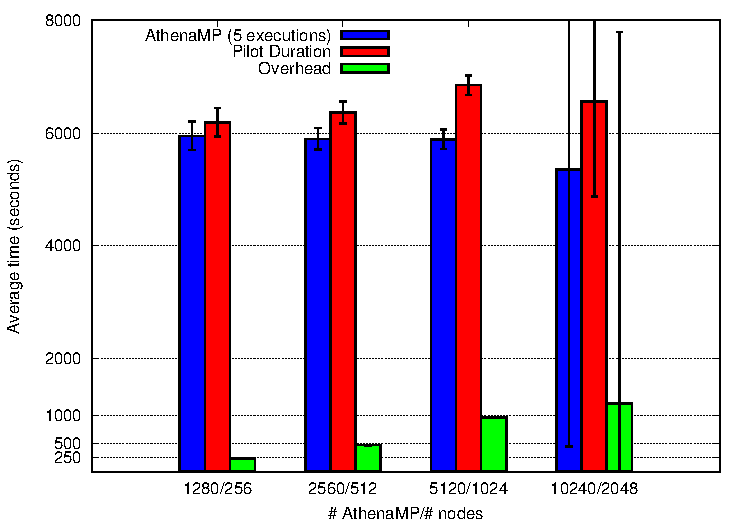
\includegraphics[height=4.5cm,width=\columnwidth]{./figures/NGE/weak2.pdf}
    \caption{Weak scalability with multiple generations: average pilot
    duration, average duration of sequential AthenaMP executions, and
    pilot's overhead for pilot with 256, 512, 1024 and 2048 nodes.}
\label{fig:weakScal2a}
\end{figure}

\vspace{-0.2in}

\subsubsection{Strong scalability}

The last experiments  study strong scalability by running the same number of
tasks for different pilot sizes. We used 2048 AthenaMP instances and  pilots
with 256, 512, 1024 and 2048 nodes. Thus, the number of AthenaMP generations is
equal to eight times the size of the smallest pilot and corresponds to the size
of the largest pilot. As a consequence, the number of consecutive generations of
AthenaMP decreases with the pilot size by generating different dynamics within
the pilots. These experiments are designed to investigate whether pilot overhead
is affected by the degree of concurrency within the pilot and/or the number of
tasks. Each AthenaMP instance simulates sixteen events as in the previous
experiment.

Fig.~\ref{fig:strongScala}  shows the average pilot duration and the average
execution time of possibly sequential AthenaMP instances.  We  notice that the
difference between the pilot duration and the AthenaMP execution times is almost
constant for all the pilot sizes, although the overall duration of the pilot
decreases linearly with the pilot size.

\begin{figure}[!htb]
        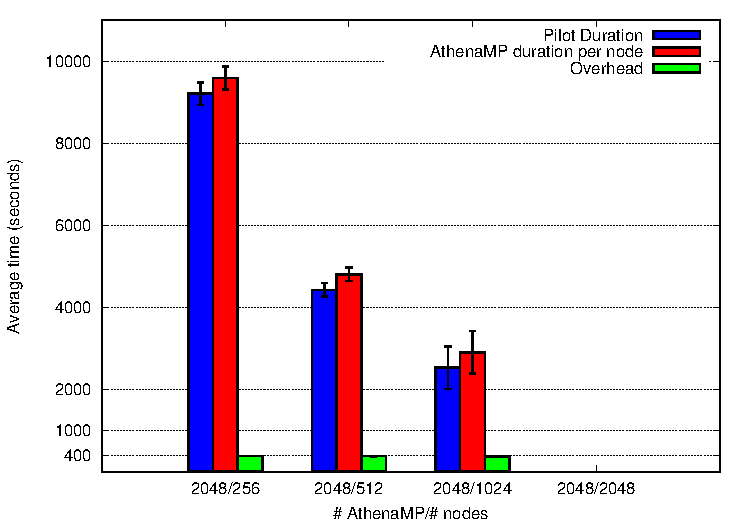
\includegraphics[height=4.5cm,width=\columnwidth]{./figures/NGE/strong.pdf}
    \caption{Strong scalability:  average pilot duration, average duration of
    sequential AthenaMP executions, and pilot's overhead for pilots with 256, 512, 1024 and 2048 nodes.}
\label{fig:strongScala}
\end{figure}

\vspace{-0.15in}



% ----------------------------------------------------------------------------
% VIII - CONCLUSIONS
% ----------------------------------------------------------------------------
\section{Conclusion}
\label{sec:conclusion}

The PanDA  system was developed to meet the scale and complexity of LHC
distributed computing for the ATLAS experiment.  In the process,  the old batch
job paradigm  of computing in HEP was  discarded  in favor of a  far more
flexible and scalable  model. The success  of PanDA  at the LHC is leading to
widespread adoption and testing by other experiments. PanDA  is the first
exascale  workload management system in HEP, already operating at a million
computing jobs per day, and processing over an exabyte of data in 2013. Next LHC
run will pose massive computing  challenges. With a  doubling of the beam
energy  and luminosity as  well as an increased  need for  simulates  data, the
data volume is expected to increase with a factor 5--6 or more. Storing and
processing  this amount of data is a  challenge   that cannot be resolved with
the currently existing  computing  resources in ATLAS\@. To resolve this
challenge, ATLAS is turning to commercial  as well as academic Cloud services
and HPCs via the PanDA system. Also the work underway is enabling the use of
PanDA by new scientific collaborations and communities as a means  of leveraging
extreme scale computing  resources with a low barrier of entry. The technology
base provided by the PanDA system will enhance the usage of a variety  of
high-performance computing resources available to basic research.


% ----------------------------------------------------------------------------
% ACKNOWLEDGEMENTS
% ----------------------------------------------------------------------------
\section*{Acknowledgements}
\label{sec:ack}

The authors would like to thank... More thanks here...

This research used resources of the Oak Ridge Leadership Computing Facility,
located in the National Center for Computational Sciences at the Oak Ridge
National Laboratory, which is supported by the Office of Science of the
Department of Energy under Contract DE-AC05-00OR22725.

What other boilerplate text is needed?




%\section*{Acknowledgment}

%The authors would like to thank... More thanks here...

% trigger a \newpage just before the given reference
% number - used to balance the columns on the last page
% adjust value as needed - may need to be readjusted if
% the document is modified later
%\IEEEtriggeratref{8}
% The "triggered" command can be changed if desired:
%\IEEEtriggercmd{\enlargethispage{-5in}}

% references section

% can use a bibliography generated by BibTeX as a .bbl file
% BibTeX documentation can be easily obtained at:
% http://www.ctan.org/tex-archive/biblio/bibtex/contrib/doc/
% The IEEEtran BibTeX style support page is at:
% http://www.michaelshell.org/tex/ieeetran/bibtex/
%\bibliographystyle{IEEEtran}
% argument is your BibTeX string definitions and bibliography database(s)
%\bibliography{IEEEabrv,../bib/paper}
%
% <OR> manually copy in the resultant .bbl file
% set second argument of \begin to the number of references
% (used to reserve space for the reference number labels box)

% ----------------------------------------------------------------------------
% REFERENCES
% ----------------------------------------------------------------------------
\bibliographystyle{plain}
\bibliography{bibliography}

% that's all folks
\end{document}
